\documentclass[nosignatures]{mscThesis}
\newcommand{\Elip}{\lsymb{$E_{LIP}$}{Linear inverted pendulum orbital energy}}
\newcommand{\Eorbit}{\lsymb{$E_{orbit}$}{Nonlinear orbital energy}}
\newcommand{\fgr}{\mathbf{F}_{gr}}
\newcommand{\fgrx}{F_{gr,x}}
\newcommand{\fgry}{F_{gr,y}}
\newcommand{\fgrz}{F_{gr,z}}
\newcommand{\cxyz}{\mathbf{c}}
\newcommand{\cxy}{\mathbf{c}_{xy}}
\newcommand{\rcmpd}{\mathbf{r}_{cmp,d}}
\newcommand{\rcmpr}{\mathbf{r}_{cmp,r}}
\newcommand{\rcmp}{\mathbf{r}_{cmp}}
\newcommand{\rcop}{\mathbf{r}_{cop}}
\newcommand{\rcopd}{\mathbf{r}_{cop,d}}
\newcommand{\icpx}{\xi_x}
\newcommand{\icpy}{\xi_y}
\newcommand{\icp}{\boldsymbol{\xi}}
\newcommand{\icpr}{\boldsymbol{\xi}_r}
\newcommand{\dotl}{\dot{\mathbf{l}}}
\newcommand{\dotld}{\dot{\mathbf{l}}_d}
\newcommand{\dotldxy}{\dot{\mathbf{l}}_{d,xy}}
\newcommand{\dotldz}{\dot{\mathbf{l}}_{d,z}}
\newcommand{\qjnt}{\mathbf{q}}
\newcommand{\dqjnt}{\dot{\mathbf{q}}}
\newcommand{\ddqjntd}{\ddot{\mathbf{q}}_d}
\newcommand{\ddqjntp}{\ddot{\mathbf{q}}_p}
\newcommand{\bs}[1]{\boldsymbol{#1}}
\newcommand{\matr}[1]{\mathbf{#1}} % undergraduate algebra version
%\newcommand{\matr}[1]{#1}          % pure math version
%\newcommand{\matr}[1]{\bm{#1}}  
\newcommand{\vect}[1]{\mathbf{#1}} % undergraduate algebra version
%\newcommand{\vect}[1]{#1}          % pure math version
%\newcommand{\vect}[1]{\bm{#1}}  
\newcommand{\cost}{J}
\newcommand{\wght}{\mathbf{R}}
\newcommand{\slct}{\mathbf{S}}
\usepackage{algorithm}
\usepackage{algpseudocode}
\usepackage{subcaption}


% replace the previous line with the next to include a signature page
%\documentclass{mscThesis}
% use the option 'nosignatures' to turn off the signatures page
%\documentclass[nosignatures]{mscThesis}
%
% Thesis data
%-For Confidential Reports, uncomment the next line, if desired change the argument. It is printed on the cover, title page and in the footer per page
%\mscConfidential{CONFIDENTIAL}
%
%-Definition of department, programme, faculty
\mscDepartment{Cognitive Robotics}%
\mscProgram{Systems and Control}
%Change if needed to
%\mscProgram{Mechanical Engineering}
\mscFaculty{Mechanical, Maritime and Materials Engineering (3mE)}%
%
%-name, date, title
\mscName{B.J. van Hofslot}%
\mscDate{\today}%
\mscTitle{Humanoid Robot Balance Control Using CoM Height Variations}%
\mscSubTitle{}%
\mscKeyWords{thesis, msc, subject}% only used in PDF properties
%
%-cover picture
\mscCoverPicture{STYLESTUFF/COVER}% to place a picture ( here the example COVER.eps) on the cover page. Comment out if no picture is to be used
%
%
%-Third party options (create text/logo on the copywrite page)
\mscThirdPartyText{The work in this thesis was supported by the Institute for Human and Machine Cognition. Their cooperation is hereby gratefully acknowledged.}
\mscThirdPartyLogo{STYLESTUFF/EXAMPLELOGO}
% NOTE: on the title page only the TU Delft logo is permitted.
%
%
% The examination committee  - Supervisors and Readers
\mscSupervisorOne{prof.dr.ir.~M.Y.~Supervisor}
\mscSupervisorTwo{Dr.ir.~M.Y.~Second Super}
%\mscSupervisorThree{}
\mscReaderOne{prof.dr.ir.~M.Y.~First Reader}
\mscReaderTwo{dr.ir.~F.S.T.~Reader-two}
\mscReaderThree{ir.~Th.~Reader-three}
%\mscReaderFour{}
%
% Finalize the thesis data
\setThesisInfo
%
% Use \includeonly{} to build only certain parts of your thesis
%\includeonly{introduction, real_chapter, empty_chapter, long_chapter}%
%
%PH Toegevoegd 24-10-2011
%allow (matlab, C++ etc) listing max 1pt flexibility between lines
\lstset{lineskip=0pt plus 1pt minus 0pt} %%
%
\begin{document}
%
%========================== Front matter ======================================
\frontmatter %
%
% Make the cover page and hell of a lot of title pages
\maketitle
%
%
% Abstract (does not appear in the Table of Contents)
\chapter*{Abstract}%

Traditional balance strategies for humans and humanoid robots are changing the \ac{CoP} position, a result of the `ankle strategy', change of body angular momentum, for example by a `hip strategy', and taking a step. For humanoid robots, a common assumption behind these strategies is that the \ac{CoM} height is constant, or at least predefined. However, height changes can be used as an input for balance control, as for example can be observed by an athlete performing a long jump. In this work, \ac{CoM} height variations are considered as an input for balance control. The results are compared with constant height approaches.

The first contribution proposes bounds on the initial states of the \ac{VHIP} from which convergence is possible, also known as capture regions. First, only a unilateral contact constraint is considered; negative \ac{CoM} acceleration cannot be smaller than gravitational acceleration. Second, \ac{CoM} height constraints are added to the model, after which a capture region can still be computed closed-form. Third, vertical acceleration constraints are added, after which capture regions are computed numerically using a bang-bang control law. The last capture region bridges the transition to the applied part of this work.

The second contribution proposes a bang-bang control law, suitable for application on humanoid robot using momentum-based control. Push recovery is tested on NASA's Valkyrie humanoid robot while the robot is standing. In simulation, an increase in recoverable push of $9$\% can be observed compared to a controller that only uses \ac{CoP}, when pushing the back of the robot. On hardware, an average increase of $7$\% can be observed for this push direction using a load sensor. Additionally, tests are conducted on hardware on Boston Dynamics' Atlas using a medicine ball on a rope, but no improvement in recovery was observed. The control method for standing push recovery is also extended for the use in walking scenarios. For Valkyrie in simulation, recovery improved the most for a push applied in the first phase of the single support state for rear and frontal push directions. 
%
% table of contents, (\toc of \toclof of \tocloflot )
\tocloflot
%
%
\include{preface}
%
% Acknowledgements
\chapter{Preface \& Acknowledgments}%
Having a background in mechanical engineering, I have always been motivated in closing the gap between theory and application on a physical system during my master's in control systems. The topic of humanoid robotics offers a very interesting, challenging, platform to dedicate my motivation to. The complex multi-body system of a humanoid robot copes with nonlinearity, hybrid dynamics, actuation limitations and plays with your human intuition. Also, humanoid robots are still physically far behind of what a human can do, which proves that there is large room for improvement. I hope in the future, robots will be able to save lives. I believe reaching out to \ac{IHMC} was the best decision to learn from and contribute to this field of research.

I would like to thank \ac{IHMC}, for giving me the opportunity to conduct research at the robotics lab. I am particularly grateful for the supervision that was given to me by Dr. Robert Griffin, Dr. Sylvain Bertrand and Dr. Jerry Pratt. I would like to thank everybody else at the robotics lab for their advice and the joy I experienced of working at the lab. 

I would also like to thank Dr. Javier Alonso-Mora from Delft University of Technology, for supervising me throughout the year I was abroad. Also, I would like to thank the assessment committee members Prof. Dr. Martijn Wisse, Dr. Tamas Keviczky and Dr. Carlos Hernandez Corbato.

I would like to thank my mother, father and two brothers, for always being supportive.

\vspace*{15mm}

Delft, University of Technology \hfill \mscname \\
\mscdate          
%
% Dedication page. 
\cleardoublepage
\thispagestyle{empty}
\vspace*{\stretch{1}}

% Put your own motto here, or dedicate your work to your Mom or whatever...
\begin{quote}
\noindent``Playing football is very simple, but playing simple football is the hardest thing there is.''
	
--- \emph{Johan Cruyff}
\end{quote}

\vspace{\stretch{3}}
\clearemptydoublepage
%
%========================== Main matter ======================================
\mainmatter
%
%
% Introduction
\chapter{Introduction} \label{chap::intro}
\section{Motivation}

Different reasons to research varying \ac{CoM} height: 
\begin{itemize}
	\item Improve behavior over rough-terrain
	\item Minimize energy consumption or mimic natural behavior
	\item Analyse the effects of height variation
	\item Extend control authority by using height variations
\end{itemize}
A common approach in humanoid robotics is to define the system as a \ac{LIP} with finite-sized foot and a mass with inertia. The ankle and the angular momentum about the \ac{CoM} can be used as control inputs to generate horizontal forces on the \ac{CoM}, often called "ankle" and "hip" strategies. Allowing for the vertical component of the \ac{GRF} to vary, more horizontal force can be generated as well.
\section{Research Objective}
In this thesis is focussed on the last two goals. Analyse the effects of height variation. Extend the control authority by using height variations. 

\section{Contributions}
\begin{itemize}
	\item Theoretic Limits on Capture
	\item Orbital Energy MPC
	\item Approaches for application on real robot
\end{itemize}
\section{Thesis Outline}



%
% A Real Chapter
\chapter{Background}\label{chap:background}
In this chapter, a brief background is given on legged systems, humanoid robotics at \ac{IHMC} and related works to \ac{CoM} height variation.
% Modeling of Walking
\section{Legged System Preliminaries}
In this section, commonly used expressions and background related to legged systems are briefly presented.
\subsection{Human Balancing Strategies}
As humanoid robots are a derivation of the human, human balancing strategies are briefly discussed. In \figref{fig:human}, human balancing strategies are shown. The `ankle strategy', `hip strategy' and stepping strategy are most commonly considered as a balancing strategy. However, the figure includes the `suspensory strategy' \cite{hasson1994clinical}, which is less commonly considered. With the `suspensory strategy', the human is in a slightly lower configuration with bend knees to have more control authority of the ankles.

Height variation is often not considered for a standing human. A reason for this might be that the human is often assumed to stand with straight legs. The goal of the `suspensory strategy' however, gives an interesting insight to the problem. If during the `suspensory strategy' the human would apply more force on the ground, such that a gain in height occurs, the effect of the `suspensory strategy' will get smaller as the legs straighten. Therefore, height variations for balance control can be a trade-off between the application of additional force and the gain in height. 
\begin{figure}
\centering
\includegraphics[width=0.5\textwidth]{STYLESTUFF/humanbalance.jpg}
\caption{Balancing strategies for a standing human \cite{hasson1994clinical}. (A) shows the `ankle strategy'. (B) shows the `hip strategy'. (C) shows the `suspensory strategy'. (D) shows the stepping strategy.}
\label{fig:human}
\end{figure}
% Ground Reference Points
\subsection{Ground Reference Points}\label{sec:grp}
In biped locomotion, the dynamics of the system are often assumed to be depending on the forces resulting from ground contact, the \ac{CoM} location and the angular moment about the \ac{CoM}. The contact forces are commonly summed up in a single \ac{GRF}, coming from a single point of application in the supporting area of the walker. Ground reference points are used to describe the dynamics of the system in a single point, using \ac{GRF} and \ac{CoM} states.

% ZMP
\paragraph{The zero moment point} is the point on the ground where the resulting \ac{GRF} does not produce any moment in the horizontal plane at the point of application \cite{sardain2004forces}. By definition, this is the point where the part of the \ac{GRF} that does not cause angular momentum around the \ac{CoM} intersects with the ground surface. The \ac{ZMP} was initially introduced in \cite{vukobratovic1969contribution}. The \ac{ZMP} is formulated as:
\begin{equation}
    \rzmp=\cxy-\frac{\fgrxy}{\fgrz}z+\frac{\taucom}{\fgrz},
\end{equation}
where $\rzmp = [x_{zmp}, y_{zmp}]^T$ is the \ac{ZMP} location, $\fgrxy=[\fgrx,\fgry]^T$ and $\fgrz$ are the horizontal and vertical components of the \ac{GRF} respectively, $\cxy = [x,y]^T$ and $z$ are the horizontal and vertical components of the \ac{CoM} Cartesian position and $\taucom = [-\tau_y,\tau_x]^T$ is the torque about the \ac{CoM} in the horizontal plane. 

In \figref{fig:zmpvscmp} the definition of the \ac{ZMP} is visualized for two different modeling choices, using both a connection between the ankle and the \ac{CoM} as a prismatic joint. In \figref{fig:3dlipfoot}, no inertia is considered around the \ac{CoM} and the \ac{GRF} $\fgr$ coming from the \ac{ZMP} intersect with the mass $m$. The difference in position between the ankle location and the \ac{ZMP} is affected by the ankle torque $\tauankle$. In \figref{fig:3dlipfootinertia}, body inertia of the system is approximated by adding a flywheel with inertia $\inert = [I_x, I_y]^T$ to the model. The \ac{GRF}, coming from the \ac{ZMP}, can be pointed away from the \ac{CoM} by using the body torque $\taucom = [\tau_x, \tau_y]^T$ as input. 

% CoP
\paragraph{The center of pressure} coincides during walking over flat ground with the \ac{ZMP} \cite{vukobratovic2004zero}. The two points however are not equal in more complex environments. The \ac{CoP} is restricted to be located in the support polygon, while the \ac{ZMP} is restricted to be located on the ground plane  \cite{sardain2004forces}. Traditionally, the \ac{CoP} is a measured quantity from a force pressure plate under the foot. In this thesis, the \ac{CoP} location is denoted as $\rcop = [x_{cop}, y_{cop}]^T$ and considered equal to $\rzmp$, as a flat contact surface is used as reference.
%The \ac{CoP} is linked to the \ac{GRF}-moment, while the \ac{ZMP} is related to the effects of external forces on the \ac{CoM} state \cite{sardain2004forces}. 
\begin{figure}
\centering
\begin{subfigure}{0.49\textwidth}
\centering
\includegraphics[width=.9\linewidth]{STYLESTUFF/3DCoPviz.png}
\caption{}
\label{fig:3dlipfoot}
\end{subfigure}
\begin{subfigure}{0.49\textwidth}
\centering
\includegraphics[width=.9\linewidth]{STYLESTUFF/3DCMPCoPviz.png}	
\caption{}
\label{fig:3dlipfootinertia}
\end{subfigure}
\caption{Ground reference points for different modeling choices. (a) The yellow cross points out the \ac{ZMP}/\ac{CoP} location. As no angular momentum is considered in the model,  the yellow cross is also the \ac{CMP}. (b) A flywheel with inertia is added to the model, the blue cross points out the \ac{CMP} location and the yellow cross the \ac{ZMP}/\ac{CoP} location.}
\label{fig:zmpvscmp}
\end{figure}

% CMP
\paragraph{The centroidal moment pivot} includes, unlike the \ac{ZMP} and \ac{CoP}, angular momentum around the \ac{CoM}  \cite{popovic2005ground}. This is defined as the point where a line passing through the \ac{CoM}, parallel to the \ac{GRF} intersects with the ground surface. Unlike the \ac{CoP}, the \ac{CMP} is not constrained to lie inside the support polygon. The \ac{CMP} is defined as:
\begin{equation}
    \rcmp=\cxy-\frac{\fgrxy}{\fgrz}z,
    \label{eq:cmp}
\end{equation}
where $\rcmp =[x_{cmp}, y_{cmp}]^T$ is the \ac{CMP} location. In \figref{fig:3dlipfootinertia} the difference between the \ac{ZMP} and \ac{CMP} is graphically explained. Note that without body inertia in the model, the points coincide, as is depicted in \figref{fig:3dlipfoot}. Equivalently, if $\taucom=0$, the points coincide as well.

%leg modeling
\subsection{Inverted Pendulum-based Models}
The line between a ground reference point and the \ac{CoM} can be modeled as an inverted pendulum. In this thesis, this line is also called the \textit{virtual leg}.

\paragraph{The linear inverted pendulum model} is widely used in walking research and especially in legged robotics \cite{kajita20013d}. The \ac{LIP} provides fast, closed-form solutions when integrating over time. In the \ac{LIP} equations of motion, the horizontal motion of the pendulum tip does not affect the pendulum length $l$:
\begin{equation}
\ddcxy=\frac{g}{l}\cxy,
\label{eq:LIPeom}
\end{equation}
where $\ddcxy$ is the horizontal \ac{CoM} acceleration. At any horizontal position, a constant leg length is considered and the motion is at a constant height $l=z_0$. In \figref{fig:3dlip} the \ac{3D} motion is visualized if the \ac{CoM} is relatively far from from the base. The pendulum base lies in the origin. Because the \ac{LIP} assumption holds, the vertical component of $\fgr$ cancels out gravity acceleration: $\fgrz=mg$.\\
\begin{figure}
\centering
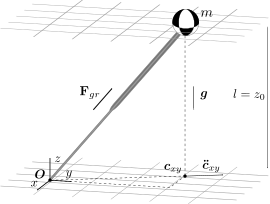
\includegraphics[width=0.5\textwidth]{STYLESTUFF/3DCoMwithoutfoot.png}
\caption{\ac{3D} motion of \ac{LIP} model.}
\label{fig:3dlip}
\end{figure}

To model body inertia of the robot, sometimes a flywheel is added to the \ac{LIP} \cite{pratt2006capture}, \cite{stephens2007humanoid}, \cite{koolen2012capturability}. By controlling the torque applied on the flywheel, the \ac{CoM} dynamics can be controlled.

% height var model
\paragraph{Height varying models} consider, unlike the \ac{LIP}, height variation of the \ac{CoM}. Three examples of such models are:
\begin{itemize}
	\item The, not linearized, inverted pendulum model \cite{kuo2005energetic};
	\item The \ac{SLIP} model \cite{liu2015trajectory};
	\item A pendulum with prismatic joint, not constrained to maintain a constant height: the \ac{VHIP} \cite{pratt2007derivation}.
\end{itemize}
The inverted pendulum model is often used in human motion research, as in \cite{kuo2005energetic}. The advantages of a \ac{LIP}, like fast, closed-form solutions to the dynamics, are often not needed. The \ac{SLIP} model originates from hopping and running robots \cite{schwind1998spring}. Deviations from the nominal height or pendulum length are modeled as mass-spring dynamics. 

Throughout this report, special focus is given to the \ac{VHIP}. In \figref{fig:3dvhip} the \ac{VHIP} is depicted. The dynamics of the point-mass can be written in two ways. One is as a function of the \ac{GRF} in \ac{2D}:
\begin{align}
	m\ddot{x} &= \fgrtwo\frac{x}{\sqrt{x^2 + z^2}},\\
	m\ddot{z} &= \fgrtwo\frac{z}{\sqrt{x^2 + z^2}} - mg,
	\label{eq:dynamicsprattstyle}
\end{align}
where $\fgrtwo=[\fgrx, \fgrz]^T$ is the \ac{GRF} of the \ac{2D}  model. Works that use this style of writing are, for example, \cite{pratt2007derivation} and \cite{koolen2016balance}.

Another way of writing the dynamics of the \ac{VHIP} is as a function of the vertical acceleration $\ddot{z}$:
\begin{equation}
	\ddcxyz = \frac{g+\ddot{z}}{z}\cxyz + \vect{g},
	\label{eq:dynamicscaronstyle}
\end{equation}
where $\vect{g}=[0,0,-g]$ is the gravity force vector. The dynamical equation can be seen as a linear time-varying system. Examples of works that use the latter dynamical description for the \ac{VHIP} are \cite{hopkins2014humanoid} and \cite{caron2018balance}. Note that the two models are identical in \ac{2D}.
\begin{figure}
\centering
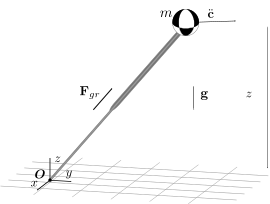
\includegraphics[width=0.5\textwidth]{STYLESTUFF/3DCoMwithoutfootVHIP.png}
\caption{\ac{3D} motion of \ac{VHIP} model.}
\label{fig:3dvhip}
\end{figure}

% Energy of Walking
\subsection{Orbital Energy \& the Capture Problem}\label{sec:ewalking}
An advantage of the \ac{LIP} is that closed-form solutions to the dynamics exists. The \ac{LIP} orbital energy is an example of such a closed-form solution. This energy can be used to determine the ability of the pendulum to converge to its unstable mode: the capture problem \cite{pratt2006capture}, \cite{koolen2012capturability}.

% LIP orbital energy
\paragraph{The linear inverted pendulum orbital energy}\label{subsec:liporbit} is originally derived in \cite{kajita1992dynamic} and shows one of the main advantages of the use of a \ac{LIP} model.  This energy reads as follows
\begin{equation}
\Elip = \int (\ddot{x}-\frac{g}{l}x)\dot{x} dt = \frac{1}{2}\dot{x}^2-\frac{g}{2z_0}x^2,
\label{eq:Elip}
\end{equation}
where $E_{LIP}$ is the \ac{LIP} orbital energy. Note that the expression resembles kinetic and potential energy: one term depends on velocity, the other on position. If $E_{LIP}>0$, the point mass will cross the horizontal position of the pendulum base with its current velocity. If $E_{LIP}<0$, the point mass will not cross the pendulum base and will have a turning point where the velocity becomes zero.

% ICP
\paragraph{The linear inverted pendulum capture point} is derived more than a decade later from $\Elip$ in \cite{pratt2006capture}. Taking $E_{LIP}=0$ and taking the square root of Equation \eqref{eq:Elip} gives
\begin{equation}
\xcplip=\sqrt{ \frac{z_0}{g}}\dot{x} 
\label{eq:cp}
\end{equation}
where $\xcplip$ is the `capture point', in this thesis referred to as the \ac{CP}. This is the point where the velocity of the point-mass is exactly driven to zero and the pendulum is upright, where neither crossing of the pendulum base ocurred nor turning of body velocity. In \figref{fig:2dicp} a \ac{2D} visual explanation is given of this point. The \ac{CP} will be used for comparison with the \ac{VHIP} capture regions later in this report.
\begin{figure}
\centering
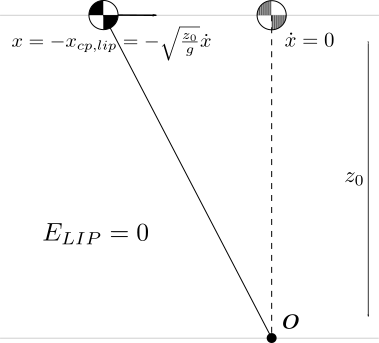
\includegraphics[width=0.4\textwidth]{STYLESTUFF/2DCP.png}
\caption{Visualization of the path to the \ac{CP}. }
\label{fig:2dicp}
\end{figure}

\paragraph{A capture region} will traditionally appear if the \ac{LIP} plus flywheel model is used \cite{pratt2006capture}, \cite{stephens2007humanoid}, \cite{koolen2012capturability}. As the control authority of the flywheel can change the \ac{CoM} dynamics, a set of capture points become reachable.

\paragraph{The instantaneous capture point} was introduced in \cite{koolen2012capturability}, which gives a slightly different description of the \ac{CP}:
\begin{equation}
\icp=\cxy+\sqrt{\frac{z_0}{g}}\dot{\mathbf{c}}_{xy} 
\label{eq:icp}
\end{equation}
where $\icp=[\icpx, \xi_y]^T$ is the \ac{ICP}. In this way, the \ac{CP} is written in environmental coordinates and can be seen as a point where to step in the environment to come to a stop. Other similar mentions to the \ac{ICP} are the extrapolated center of mass \cite{hof2008extrapolated} and the \ac{DCM} \cite{takenaka2009real}. 
\paraskip
For planning and control, the time derivative is often taken of the \ac{ICP}: the \ac{ICP} dynamics \cite{koolen2012capturability}. This time derivative can be written as a function of the current \ac{ICP} location and a ground reference point:
\begin{equation}\label{eq:icpdyn}
\dot{\icp}=\sqrt{ \frac{g}{z_0}}(\icp-\vect{r})
\end{equation}
where $\dot{\icp}$ is the \ac{ICP} velocity and $\vect{r}$ is a ground reference point, depending on modeling choices as discussed in Section \ref{sec:grp}.

% Boundedness
%\paragraph{The boundedness condition}\label{sec:boundedness} \cite{lanari2014boundedness} includes the effects of the motion of the ground reference point in the capture problem. The solution of $x_u$, a point that also coincides with the \ac{ICP}, reads as:
%\begin{equation}
%x_u(t,r) = e^{\omega_0(t-t_0)}x_u(t_0) -\omega_0 \int_{t_0}^t e^{\omega_0(t-\tau)}r(\tau)d \tau,
%\end{equation}
%where $r(t)$ is the trajectory described by the used ground reference point, the virtual base of the pendulum. The boundedness condition reads as follows: if the the future input $r(t)$ results in convergence of the \ac
%{CoM} to the unstable mode, the following equality holds:
%\begin{equation}
%x_u(t_0) = \omega_0 \int_{t_0}^{\infty} e^{-\omega_0(\tau-t_0)}r(\tau)d \tau.
%\end{equation}
%The initial condition, which is equal to the \ac{ICP}, has to be related to $r(t)$ by this expression.

%nonlinear orbital
\paragraph{Orbital energy with height variation}\label{subsec:nonorbit} is more difficult to derive than its linear counterpart.  Examples of attempts to include \ac{CoM} height variations in the solution to the dynamics are the time-varying \ac{DCM} \cite{hopkins2014humanoid}, the orbital energy under a virtual constraint \cite{pratt2007derivation} and the height varying boundedness condition \cite{caron2018balance}. These works are discussed in Section 
\ref{sec:relatedworksheight}, since they are highly related to the research of focus.

% Control Framework IHMC
\section{Humanoid Robotics at IHMC}\label{sec:ihmc}
To support the methods and results presented later in this thesis, this section presents a brief background on humanoid robotics at \ac{IHMC}. Most algorithms are written in Java and simulations are run in \ac{SCS}.
%robots
\subsection{Robots}
There are two humanoid robots present at the institute at the moment of writing: Boston Dynamics' Atlas \cite{koolen2016design}, \cite{kuindersma2016optimization} and NASA's Valkyrie \cite{radford2015valkyrie}. An important difference between the two robots is that Atlas is hydraulically actuated, while Valkyrie relies on electric series elastic actuators. The actuation of Atlas is in general more powerful, which allows the robot to take higher steps. Valkyrie on the other hand, has more precise torque sensing, which is important for torque control on the robot. This ties to a similarity between the robots: both robots are torque controlled. Using a control framework, the actuators of the robots can be controlled using measured and reference torque. In \figref{fig:robots}, the two robots are shown.
\begin{figure}
\centering
  \begin{subfigure}{0.49\textwidth}
  \centering
  \includegraphics[width=.6\linewidth]{STYLESTUFF/AtlasOld1.png}
   \caption{}
    \label{fig:atlas}
  \end{subfigure}
  \begin{subfigure}{0.49\textwidth}
    \centering
  \includegraphics[width=.6\linewidth]{STYLESTUFF/Valkyrie1.png}
  \caption{}
   \label{fig:valkyrie}
  \end{subfigure}
  \caption{(a) Atlas \cite{oldatlas} and (b) Valkyrie \cite{valkyrie} walking over an un-even cinder block field at \ac{IHMC}. }
  \label{fig:robots}
\end{figure}

% planning
\subsection{Planning}
In contrary to running, with walking there is a state in every cycle with two feet in contact with the ground. This is the \ac{DS} state and the state where only one leg is on the ground is the \ac{SS} state. Additionally, other states within either the \ac{DS} or \ac{SS} state are considered, like toe-off in the transition from \ac{DS} to \ac{SS}. In \ac{SS}, the leg in contact with ground is the support leg and the foot taking a step is the swing leg. The transition between those states and the duration in each state play an important role in the generation of a dynamic plan. Planning of the robots motion is conducted by separating footstep planning from dynamic planning. The dynamic plan is in this case an \ac{ICP} reference trajectory \cite{seyde2018inclusion}.
%footstepplan
\paragraph{Footstep planning} is the generation of a sequence of footsteps for the robot to follow. A Light Detection and Ranging sensor on the head of the robot provides terrain information. One way to generate a footstep plan is to let the user define each footstep via a graphical user interface. Via relatively simple algorithmic checks on for example kinematic reachability, the user interface can show whether a to be placed footstep is feasible or not. To make this process more autonomous, recently developments have been made in the creation of a footstep planner based on a A* search algorithm. 
%icpplanning
\paragraph{Instantaneous capture point planning}\label{subsec:icpplan} is the generation of a dynamic plan for the robot. It relies on the solution to the linear differential equation of the \ac{ICP} dynamics of Equation \eqref{eq:icpdyn}:
\begin{equation}\label{eq:icpsol}
	\icp(t)=e^{\omega_0t}(\icp_0- \vect{r}_0) + \vect{r}_0,
\end{equation}
where $\omega_0=\sqrt{\frac{g}{z_0}}$ is the natural frequency of the \ac{LIP} and $\icp_0$ and $\vect{r}_0$ are the initial \ac{ICP} and ground reference point location or the \textit{knot-points}. This equation assumes that the location of the ground reference point is constant. 

Under the assumption of constant ground reference point locations, the ground reference knot-points, multiple methods have been developed over the years and improvements are being made. The most traditional \ac{ICP} reference trajectory is calculated with a single \ac{ZMP} knot-point \cite{englsberger2012integration} for each footstep. For each \ac{ZMP} knot-point, an \ac{ICP} knot-point is computed by integrating the \ac{ICP} dynamics backwards in time from the last footstep to the first. Using Equation \eqref{eq:icpsol}, the local \ac{ICP} reference value can be computed at any time instance within the plan. 

The above mentioned method is extended in \cite{englsberger2014trajectory}, where multiple \ac{CMP} knotpoints per foot are considered and \ac{SS} and \ac{DS} transitions are interpolated using splines. In the most recent improvements, continous \ac{CMP} reference trajectories are used for the generation of the \ac{ICP} trajectory \cite{seyde2018inclusion}. An estimate of the angular momentum generated during the walking motion is incorporated in the generation of the \ac{CMP} reference. At the time of writing, the latter method is the one currently in use, and which is used for the experiments in Chapter \ref{chap:walking}.
% icp control
\subsection{Instantaneous Capture Point Control}\label{sec:icpcontrol}
Based on a \ac{CMP} and \ac{ICP} reference trajectory, the following proportional control law is used to generate a desired \ac{CMP}:
\begin{equation}
    \rcmpd=\rcmpr + \mathbf{k}_{\xi}(\icp-\icpr),
    \label{eq:rcmpd}
\end{equation}
where $\rcmpd$ is the desired \ac{CMP}, $\rcmpr$ and $\icpr$ are the reference \ac{CMP} and \ac{ICP} from the \ac{ICP} planner respectively and $\mathbf{k}_{\xi}$ is the \ac{ICP} gain. From $\rcmpd$, the desired horizontal linear momentum rate of change is computed:
\begin{equation}\label{eq:dotldxy}
    \dotldxy = \frac{\cxy-\rcmpd}{z_0}mg,
\end{equation}
where $\dotldxy$ is the desired horizontal linear momentum rate of change, which is the desired horizontal force on the \ac{CoM} of the robot. This value is send to the whole-body \ac{QP}. Note that this value is computed based on the \ac{LIP} equations of motion. 

% momentum control
\subsection{Momentum-based Whole-body Control}
The desired horizontal linear momentum rate of change $\dotldxy$, the output of \ac{ICP} control, is one of the inputs for the the whole-body \ac{QP}. The whole-body \ac{QP} finds desired joint accelerations and desired \ac{GRF}, which are translated to desired joint torques by a Newton-Euler inverse dynamics algorithm.
%centroidal
\paragraph{Centroidal dynamics} \cite{orin2013centroidal} describe the dynamics on and about the \ac{CoM} of the robot as a result of external forces like gravity and \ac{GRF}. To find the \ac{CoM} dynamics for the robotic chain of the humanoid, a short introduction is given to joint to end-effector mapping. The mapping between joint velocities and end-effector motion plays a crucial role in any robotic system:
\begin{equation}\label{eq:jacobian}
\matr{T}=\begin{bmatrix}\bs{\omega} \\ \bs{\upsilon} \end{bmatrix} = \matr{J}(\qjnt)\dqjnt \in \mathbb{R}^6,
\end{equation}
where $\dqjnt$ are the joint velocities, $\matr{J}(\qjnt)$ is the Jacobian that maps joint velocities to the end-effector twist $\matr{T}$. The twist consist of the angular velocity $\bs{\omega} \in \mathbb{R}^3$ and the linear velocity $\bs{\upsilon} \in \mathbb{R}^3$. A basis for momentum-based whole-body control is the use of centroidal momentum:
\begin{equation}
\vect{h}=\begin{bmatrix}\vect{k} \\ \vect{l} \end{bmatrix} =\matr{A}(\qjnt)\dqjnt \in \mathbb{R}^6,
\end{equation}
 where $\matr{A}=\matr{I}\matr{J}$ is the inertia matrix $\matr{I}$ times the jacobian. The centroidal momentum $\vect{h}$ consists of the angular part $\vect{k} \in \mathbb{R}^3$ and the linear part $\vect{l} \in \mathbb{R}^3$. The time derivative of the centroidal momentum, the centroidal momentum rate of change, is the constraint on the dynamics of the robot in the \ac{QP} currently in use \cite{koolen2016design}:
\begin{equation}
\dot{\vect{h}}=\begin{bmatrix}\dot{\vect{k}}\\ \dot{\vect{l}} \end{bmatrix} =\matr{A}\ddot{\vect{q}} +\dot{\matr{A}}\dot{\vect{q}} = \matr{W}_g + \sum_i\matr{W}_{gr,i} + \sum_i \matr{W}_{ext,i}, 
\end{equation}
where $\matr{W}_g$ is the gravitational wrench and $\sum_i\matr{W}_{gr,i}$ the wrench exterted by the total \ac{GRF}, as a sum from the wrench at each contact point considered. The other external wrenches $\sum_i \matr{W}_{ext,i}$ can be caused for example by other contacts than ground. These are considered zero in this thesis: $\sum_i \matr{W}_{ext,i}=\vect{0}$.
%qp
\paragraph{The whole-body quadratic program} \cite{koolen2016design} optimizes between momentum rate objectives and motion objectives to find desired joint accelerations and desired \ac{GRF}. The optimization is formulated as follows:
\begin{equation}
\begin{array}{rlcl}
\displaystyle \min_{\bs{\ddot{q}}_d,\bs{\rho}} & \multicolumn{3}{l}{J_{\bs{\dot{h}}_d} + J_{\bs{J}} + J_{\bs{\rho}} + J_{\bs{\ddot{q}}_d} } \\%+ J_p} \\
\textrm{s.t.} & \matr{A}\ddqjntd + \dot{\matr{A}}\dqjnt = \matr{W}_g + \matr{Q}\bs{\rho}+\sum_i\matr{W}_{ext,i}\\
&\displaystyle \bs{\rho}_{min} \leq \bs{\rho}\\
&\ddot{\qjnt}_{min} \leq \ddqjntd \leq \ddot{\qjnt}_{max},
\end{array}
\end{equation}
where $\ddqjntd$ are the desired joint accelerations, $\matr{Q}\bs{\rho} = \sum_i\matr{W}_{gr,i}$ is the basis vector matrix $\matr{Q}$ times the basis vector multipliers $\bs{\rho}$. The basis vector matrix $\matr{Q}$ consists of all basis vectors of the wrench cones from each ground contact point. In \figref{fig:wrenchcone}, the wrench cone for a single ground contact point is visually explained. Currently, there are $4$ ground contact points considered for each foot of the robot.
\begin{figure}
\centering
\includegraphics[width=0.4\textwidth]{STYLESTUFF/wrenchcone.png}
\caption{Approximation of the wrench cone with basis vectors $\boldsymbol{\beta}_{ij}$ for ground contact point $i$. The linear part of the ground reaction wrench, $\vect{f}_i$ in the drawing, is a positive multiplication of the basis vectors and lies inside the wrench cone \cite{koolen2016design}. }
\label{fig:wrenchcone}
\end{figure}
The minimum $\bs{\rho}_{min}$ has to be at least zero, because of the unilateral contact constraint; the robot can only push with its feet on the ground. The total cost $J$ is composed of the following cost terms:
\begin{equation*}
\begin{array}{rlcl}
$Momentum rate objective cost:$ & J_{\dot{\vect{h}}_d}= \wght_{\dot{\vect{h}}_d}||\matr{A}\ddqjntd + \dot{\matr{A}}\dqjnt - \dot{\vect{h}}_d||^2\\
$Motion objective cost:$ & J_{\matr{J}_m} = \wght_{\matr{J}_m}||\matr{J}_m\ddqjntd-\vect{p}||^2\\
$Contact force cost:$ & J_{\bs{\rho}}=\wght_{\bs{\rho}}||\bs{\rho}||^2 \\
$Joint acceleration cost:$ & J_{\ddqjntd} = \wght_{\ddqjntd}||\ddqjntd ||^2 \\
%$Privileged configuration cost:$ & J_p = \wght_p||(\matr{I} - \matr{J}_t^{\dagger}\matr{J}_t)\ddqjntd - \ddqjntp||^2,
\end{array}
\end{equation*}
where the weighting terms $\wght$ can have a selecting function as well. For example, the centroidal momentum rate of change objective $J_{\dot{\vect{h}}_d}$ only consists of the linear part and is only affected by the desired linear momentum rate of change $\dotld$. The motion task jacobian $\matr{J}_m = [\matr{J}_1^T\quad...\quad\matr{J}_N^T]^T$ consists of all concatenated jacobians that map either joint acceleration to end-effector motion, as in Equation \eqref{eq:jacobian} or joint acceleration to joint acceleration. The motion objective vector $\vect{p} = [\vect{p}_1^T\quad...\quad\vect{p}_N^T]^T$  consists of PD-controlled desired accelerations, coming for example from trajectory tracking of the swing leg or maintaining the upper-body orientation. %The last cost term $J_p$ is determined by the privileged joint accelerations $\ddqjntp$. Here is $\matr{J}_t$ the all-task jacobian consisting of both the momentum rate objective, as well as the motion objectives. The damped Moore-Penrose pseudo-inverse  $\matr{J}_t^{\dagger} = \matr{J}_t^T(\matr{J}_t\matr{J}_t^T +\mu^2)^{-1}$ with $\mu>0$ is used in the null-space projector $(\matr{I} - \matr{J}_t^{\dagger}\matr{J}_t)$, which projects the priviliged acceleration objective in the null-space of the primary task jacobian $\matr{J}_t$. This can for example be used in singularity avoidance, where the priviliged accelerations are used to determine the configurarion of the robotic chain.  

An important note considering the research of focus is the generation of vertical \ac{CoM} motion of the robot. The desired linear momentum rate of change $\dotld$ consists, next to its horizontal component of Equation \eqref{eq:dotldxy}, of a vertical part:
\begin{equation}
\dotldz =m(k_p(z_r-z) - k_d\dot{z}), 
\label{eq:defaultheightcontrol}
\end{equation}
where $k_p, k_d$ are the PD-control gains and $z_r$ is the reference height coming from a reference trajectory. Decision variables for this trajectory are for example kinematic reachability and height changes in terrain, but maintaining the robot's balance is \textit{not} a part of those decision variables.


\paragraph{Inverse dynamics} translate desired joint accelerations and end-effector wrenches to desired joint torques. Desired joint torques $\bs{\tau}_d$ are calculated via a revursive Newton-Euler algorithm using the solution of whole-body \ac{QP}: $\ddqjntd$ and $\bs{\rho}$.
\begin{equation}
    \bs{\tau}_d = \matr{M}(\qjnt)\ddqjntd + \matr{C}(\qjnt,\dqjnt)\dqjnt + \matr{G}(\qjnt) + \matr{J}^T \vect{W}_{gr}.
\end{equation}
With the desired joint torques, the actuators of the robot are PD-controlled using a electrical current as input and joint torque and joint velocity measurements.

A high-level overview of the control framework is shown in \figref{fig:framework}. The `high level controller' block consists for example of the \ac{ICP} controller of Section \ref{sec:icpcontrol} and the height control law of Equation \eqref{eq:defaultheightcontrol}.
\begin{figure}[h]
\centering
\includegraphics[width=0.8\textwidth]{STYLESTUFF/controlframework.png}
\caption{High-level overview of the control framework \cite{koolen2016design}. }
\label{fig:framework}
\end{figure}

% CoM Height Variation
\section{Related Works}\label{sec:relatedworksheight}
In this short literature survey, the scope is not limited to only the use of vertical \ac{CoM} motion in balance control. Other goals of improvement, like improving dynamic planning for motions over rough-terrain or for more human-like motions, are discussed as well. The models and strategies used in these works can be insightful for the problem considered in this thesis.

Traditionally, vertical \ac{CoM} motion is generated through PD-control as in Equation \eqref{eq:defaultheightcontrol} \cite{kajita2003resolved, koolen2016design}: a dynamic reference plan exists, often based on the LIP model, and height variations are considered as disturbances on the model considered in the dynamical plan. Reasons to use height variations here include the guarantee of \textit{kinematic feasibility}: height variation allows the robot to step up platforms, and allows the robot to take larger steps. A noteworthy, more unique, example of height variation in non-predictive control is walking with straighter legs as in \cite{griffin2018straight}. The motivation in this work is to let the robot walk more \textit{human-like}, which could have more underlying benefits, such as kinematic reachability and metabolic energy consumption \cite{wang2012optimizing}.

%var height terrain
\subsection{Dynamic Planning \& Walking Pattern Generation}
Because the constant height assumption of the \ac{LIP} is constraining the dynamics of the robotic system, efforts have been made to incorporate CoM height variation in the generation of a dynamic plan. Instead of using a LIP model, a more complicated model is used. \textit{Expected} height variations of the CoM can be incorporated in the dynamic planning problem, which improves the \textit{dynamic feasibility} of the plan. In theory, the reference dynamics are closer to the real dynamics of the robot. Deviations from the \ac{LIP} in the \ac{CoM} reference can be incorporated in the plan. These deviations can come for example from an un-even terrain, or a human-like walking pattern.

An example of incorporating height variations in terrain in the dynamic planning problem can be found in \cite{englsberger2013three}, which is an extension of \ac{ICP} planning as in Section \ref{subsec:icpplan}. Additional reference points, similar to ground reference points as in Section \ref{sec:grp}, are designed and used in the planning method. The drawback of this method is that still a linearized model is considered and the trajectories between footsteps for the dynamical plan are constrained to be straight lines. 

Another work improved this latter aspect by introducing the time-varying \ac{DCM} \cite{hopkins2014humanoid}. The natural frequency of the \ac{LIP} was made time-varying, such that the \ac{DCM} became time-varying. However, a closed-form solution using this method was not available anymore and a dynamic plan was computed numerically.

The methods presented in \cite{brasseur2015robust} and \cite{kajita2017biped} also show the objectives of walking with straighter legs in the dynamic planning problem. The objective in the optimization in \cite{brasseur2015robust} is to let the robot walk with the straightest legs as possible at any time. In \cite{kajita2017biped}, a \ac{2D} walking pattern is generated for walking with straighter legs. The third dimension is added, under the assumption that the dynamics in the sagittal plane and the coronal plane can be decoupled. 
%balance
\subsection{Balance Control}\label{subsec:heightbalance}
A very recent objective is the specific use of \ac{CoM} height variation in \textit{balance control}. Traditional balance control strategies are taking a step, movement of the \ac{CoP}, also known as `ankle strategies' and, to a lesser extent, changing the angular momentum about the \ac{CoM}, for example: `hip strategies'. Recently, efforts have been made to incorporate vertical \ac{CoM} motions as an additional strategy for balance control. This is the research of focus in this report.

In this section, the following three publications that consider height variations as control input for balance are discussed. The work proposed by: Koolen, Posa \& Tedrake in \cite{koolen2016balance},  Gao, Jia \& Fu in \cite{gao2017increase} and  Caron \& Mallein in \cite{caron2018balance}:

% 2D polynomial
\paragraph{Koolen et al.} propose a \ac{2D} \ac{MPC} law, based on the \ac{VHIP} orbital energy proposed in \cite{pratt2007derivation}. This energy reads as follows:
\begin{equation}\label{eq:evhip}
    E_{VHIP}  = \frac{1}{2}\dot{x}^2\bar{f}^2(x)+gx^2f(x) - 3g\int_{x_f}^{x} f(\xi)\xi d\xi = \frac{1}{2}\dot{x}_f^2\bar{f}^2(x_f)+gx_f^2f(x_f),
\end{equation}
where $E_{VHIP}$ is the \ac{VHIP} orbital energy. The virtual constraint $z=f(x)$ is used to make a closed-form solution possible for the energy. Furthermore, $\bar{f}(x)=f(x)-f'(x)x$. Unlike its \ac{LIP} cousin, this \ac{2D} orbital energy allows for \ac{CoM} height variation. Note that filling in a constant value for the function, $f(x)=z_0$, rewrites to the \ac{LIP} orbital energy.

The function $f(x)$ is constrained to be a cubic polynomial by Koolen et al. in \cite{koolen2016balance}. Using this description, four constraints are presented, which are used in a matrix to solve for the polynomial constants. There is one constraint on the final height, one constraint on the initial height, one on the initial direction and one constraint on conservation of $E_{VHIP}$. The final position of the polynomial trajectory is above the \ac{CoP} and the final velocity is zero, such that the resulting polynomial trajectory is a \textit{capture trajectory}. 

Similar to the capture regions of \cite{pratt2006capture}, \textit{regions of attraction} for this controller are investigated: initial states in which this controller is still able to let the \ac{VHIP} converge to the unstable equilibrium. However, there are no kinematic constraints taken into account, such that the polynomial trajectories can become unrealistically high above the ground. Though, the analytic solution for the capture trajectory guarantees fast computation times, which allow for the use in \ac{MPC}.

\paragraph{Gao et al.} present different \ac{2D} multi-step strategies to use vertical motion in balance control in \cite{gao2017increase}. An example is the lowering of the \ac{CoM} height in the current step, to exert more force and raise the \ac{CoM} in the next step. In this way, the pendulum can stop closer to the current position than with a \ac{LIP} trajectory. Furthermore, the natural frequency of the \ac{LIP} is adjusted for the added vertical acceleration. To make the dynamical model closed-form solvable over time, a constant height is considered, as the deviations from the initial height are considered as relatively small.

% boundedness
\paragraph{Caron \& Mallein} propose a \ac{3D} \ac{MPC} law in \cite{caron2018balance}, based on a height varying version of the boundedness condition from \cite{lanari2014boundedness}. In \cite{lanari2014boundedness}, the boundedness condition is based on the \ac{LIP} and presents a similar expression as the \ac{ICP}, but takes a time-varying ground reference point trajectory into account.  By using a time varying natural frequency of the pendulum $\omega(t)$, Caron \& Mallein combine the boundedness condition with the time-varying \ac{DCM} of \cite{hopkins2014humanoid}. By the nonlinearity of the problem, it is initially hard to solve real-time. The problem function is reformulated and written as a function of an inverse of time, rather than as a function of time. Also, the capture trajectory is divided in $10$ segments, which are considered to have a piece-wise time-invariant natural frequency. The resulting problem is solved using a nonlinear solver.

This work is expanded in \cite{caron2018capturability}. The problem is extended from `0-step' capture problems to multi-step problems. The problem formulation is rewritten and sequential quadratic programming is used to allow for fast computation times, which makes the multi-step problem solvable real time.

\subsection{Discussion}
The related works show that the use of \ac{CoM} height variations in dynamic planning is a relatively longer existing research than the use of  vertical \ac{CoM} motion in balance control. However, the difference between dynamic planning and \ac{MPC} can be small. The most notable difference between the two is that with \ac{MPC} replanning is conducted every control tick, while with dynamic planning this happens fewer times. Replanning every control tick allows to adjust the dynamic plan for disturbances applied on the system. The similarity between the two is that, in the works mentioned, both use a \ac{VHIP} or an adjusted \ac{LIP} model for computing the predicted dynamics of the system.

When going from the \ac{LIP} to the \ac{VHIP}, the problem arises of losing the explicit solution to the dynamics. To avoid large computation times due to numerical integration, in the works related to balance control constraints are introduced to allow for faster solutions. More specifically, Koolen et al. constrain the \ac{2D} vertical position of the \ac{VHIP} to be a cubic polynomial function of its horizontal position. Gao et al. consider an adjusted constant natural frequency for the \ac{LIP} model to account for vertical acceleration. Caron et al. use piece-wise time-invariant natural frequencies to obtain fast solutions. Furthermore, the kinematic constraints of the robot, such as a maximum leg length, are approximated with a minimum and maximum \ac{CoM} height.

Also, the works present no application of the controllers in a control framework to control humanoid robots. Therefore, the question remains what the advantages are of the presented \ac{MPC} law compared to using a \ac{LIP}-based proportional controller for example. In Chapter \ref{chap:standing} and Chapter \ref{chap:walking} of this report, \ac{CoM} height variations in balance control are compared with constant height approaches on humanoid robots.

Comparable with the \ac{LIP}-based `capture regions' in \cite{pratt2006capture}, \cite{koolen2012capturability} and `stable regions' \cite{stephens2007humanoid},  Koolen et al. investigate `regions of attraction' for the unconstrained \ac{VHIP} orbital energy trajectories. Traditional `capture regions' consider inertia about the \ac{CoM} to control the \ac{CP}. The \ac{VHIP} `regions of attraction' use \ac{CoM} height variation as a control input. The `regions of attraction' show an interesting insight in capture regions of the \ac{VHIP} model. However, only a constraint of contact unilaterality is considered and no additional constraints are introduced to take kinematic and torque limits of the robot into account. Also, the trajectory cannot have any desired shape and is constrained by the polynomial function.

In the next chapter, capture regions are presented for the \ac{VHIP} model, by considering additional constraints. Like in the approach of Caron et al., constraints on the kinematics and dynamics of the system are approximated with a constraint on vertical position and acceleration.
%
% Another appendix chapter
\chapter{Theory: Variable Height Inverted Pendulum Capture Regions}\label{chap:regions}
Considering the \ac{VHIP}, bounds on the set of states from which convergence is possible can be derived. The following works present an equivalent study: the \ac{LIP} plus flywheel \textit{capture regions} in \cite{pratt2006capture}, stable regions \cite{stephens2007humanoid} and regions of attraction for the \ac{VHIP} orbital energy controller in \cite{koolen2016balance}. In this chapter, the term capture region is used. Furthermore, recovery is considered within the current step, which is equivalent to `0-step' capture in \cite{koolen2012capturability}. For comparison with the \ac{LIP} capture regions and for simplicity, the initial vertical velocity of the \ac{VHIP} is set to zero.

The following capture regions for the \ac{VHIP} with zero initial vertical velocity are covered in this chapter:
\begin{itemize}
	\item \textit{Analytic} capture regions based on the constraint of unilateral contact force only.
	\item \textit{Analytic} capture regions after addition of height constraints.
	\item \textit{Numeric} capture regions after addition of vertical force constraints.
\end{itemize}
Furthermore, the presented capture regions are compared with \ac{LIP} plus flywheel capture regions.

%Unilateral
\section{Unilateral Contact Constraint}
If a constraint on unilateral contact is considered, the virtual leg of the \ac{VHIP} can only apply a force on the ground of greater than or equal to zero and $\ddot{z}>g$ in the \ac{VHIP} dynamics in Equation \ref{eq:dynamicscaronstyle}. If an extremum is taken of zero leg force, the point-mass of the \ac{VHIP} follows a \textit{ballistic} trajectory, after which is reaches the ground at the ballistic touchdown point. The time after which the point-mass touches the ground is:
\begin{equation}\label{eq:tbal}
	t_{bal} = \sqrt{\frac{2z_0}{g}}.
\end{equation}
The horizontal, ballistic, touchdown location is:
\begin{equation}
	x_{bal}= \dot{x}_0t_{bal}=\dot{x}_0\sqrt{\frac{2z_0}{g}}. 
	\label{eq:xbal}
\end{equation}
This point compares to the \ac{CP} as:
\begin{equation}
    x_{bal}=\sqrt{2}x_{cp}
\end{equation}

This can also be reasoned from a virtual leg force perspective, as no horizontal energy is subtracted from the point-mass during its travel. Using this problem formulation and inserting a final velocity in the \ac{LIP} orbital energy Equation \eqref{eq:Elip} gives:
\begin{equation}
   x_{bal}^2 = \frac{z_0}{g}\big(\dot{x}_0^2 + \dot{x}_f^2\big), 
\end{equation}
where $\dot{x}_f$ is the final horizontal velocity of the \ac{CoM}. If a ballistic trajectory is considered, the horizontal velocity is not affected until touchdown, so $\dot{x}_0=\dot{x}_f$. The solution to $x_{bal}$ is equal to Equation \ref{eq:xbal}.

The unilateral contact constraint capture region is explained as follows. At touchdown, the virtual leg can apply an impulse such that $\dot{x}_f$ becomes zero. After this, the point-mass can be risen to its original height again, without influencing the horizontal dynamics, which are zero. This is one bound on the region. On the other side of the region, when the point-foot position is infinitely close to the point-mass, the virtual leg can apply an infinite force to let the horizontal velocity become zero. After this, the point-mass can be lowered again to its default height. The capture positions spanned between these two bounds reads as follows:
\begin{equation}
x_{cp,unilateral} \in \Bigg(0, \dot{x}_0\sqrt{\frac{2z_0}{g}} \Bigg],
\label{eq:xcpuni}
\end{equation}
where $x_{cp,unilateral}$ is a unilateral contact constrained capture position. In \figref{fig:cpbal} this region and how this compares to the \ac{CP} is visualized. With gray plots, made with the method of \cite{koolen2016balance}, it can be observed how the trajectories can become very high, when approaching the left side of the bound. The proof for that the ballistic touch down point is an outer bound on the unilateral contact constrained capture region can also be found in \cite{koolen2016balance}.

\begin{figure}
\centering
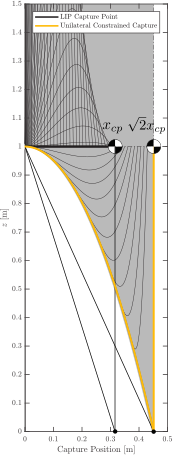
\includegraphics[width=3.0in]{STYLESTUFF/CPvsBalistic2.png}
\caption{Unilateral contact constrained capture region (gray area). The thin black lines visualize possible intermediate trajectories and are made with the method of \cite{koolen2016balance}.}
\label{fig:cpbal}
\end{figure}

%% Height Constrained
\section{Height Constraint}
Under the assumption that kinematic limits of the robotic system can be approximated with a minimum and maximum \ac{CoM} height, in this section a minimum and maximum height constraint are added to the unilateral contact constraint capture region of the previous section. All capture points that will be discussed are a combination of impacts, ballistic trajectories and \ac{LIP} capture trajectories, such that a closed-form solution becomes available. 
%minheight
\subsection{Minimum Height}
First the impact influence capture point is presented, which is used to formulate a capture point following the minimum height constraint.
\paragraph{The impact influenced capture point} is computed as follows. Temporally, the constraint on zero initial vertical velocity is neglected and the initial vertical velocity is set to a negative value. Under the assumption that this vertical velocity is directly driven to zero after an impact of the leg, the resulting capture position can be computed as follows:
\begin{equation}
x_{cp,I} = \sqrt{\frac{z}{g}}(\dot{x}_0+\dot{x}_I),
\end{equation}
where $x_{cp,I}$ is the impact influenced capture point and $\dot{x}_I$ is the added velocity generated by an impact. This added velocity in terms of vertical velocity is written as:
\begin{equation}
x_{cp,I} = \sqrt{\frac{z_0}{g}}\Big(\dot{x}_0-\frac{x_{cp,I}}{z_0}\dot{z}_I\Big),
\end{equation}
where $\dot{z}_I$ is the vertical impact generated by the virtual leg. Under the assumption that the vertical velocity is driven to zero instantaneously by the impact, $\dot{z}_I=-\dot{z}_0$. Again, writing this point not as a function of itself, leads to:
\begin{align}\label{eq:xcpimpact}
x_{cp,I} &= \frac{\sqrt{\frac{z_0}{g}}}{1+\frac{\dot{z}_I}{z_0}\sqrt{\frac{z_0}{g}}}\dot{x}_0,\\
			&= \frac{z_0}{\sqrt{z_0g}-\dot{z}_0}\dot{x}_0.
\end{align}

\paragraph{The capture position under the minimum height constraint} is computed as follows. Using Equation \ref{eq:tbal}, the ballistic trajectory until the minimum height has as final height velocity:
\begin{equation}
	\dot{z}_{\zmin} = -gt_{bal,z_{min}} = -g\sqrt{\frac{2\delta{\zmin}}{g}} = -\sqrt{2g\delta{\zmin}},
\end{equation}
where $t_{bal,\zmin}$ and $\dot{z}_{\zmin}$ are the time and vertical velocity at the minimum height constraint and $\delta{\zmin}=z_0-z_{min}$. Plugging this vertical velocity in the impact influenced capture point of Equation \eqref{eq:xcpimpact} brings:
\begin{equation}
	x_{cp,I}(z_{min}, \dot{z}_{\zmin})= \frac{\zmin}{\sqrt{\zmin}+\sqrt{2g\delta{\zmin}}}\dot{x}_0.
\end{equation}
The capture point under a minimum height constraint is:
\begin{equation}
	x_{cp,\zmin} =x_{bal,\zmin}+x_{cp,I}(z_{min}, \dot{z}_{\zmin}) ,
\end{equation}
where  $x_{bal,zmin}$ is the horizontal position at the end of the balistic part. This results in the following equation for the capture position under the minimum height constraint:
\begin{equation}
 x_{cp,\zmin}=\Bigg(\sqrt{\frac{2\delta{\zmin}}{g}} +\frac{\zmin}{\sqrt{\zmin g}+\sqrt{2g\delta{\zmin}}}\Bigg)\dot{x}_0.
\end{equation}
%maxheight
\subsection{Maximum Height}
With an initial impact of the leg of such magnitude that the resulting apex of the point-mass does not violate the maximum height constraint, a capture position under a maximum height constraint can be derived. To calculate the allowed size of the initial impact, the following equality of kinetic and potential energy is used:
\begin{align}
 	\frac{1}{2}m\dot{z}_I^2 &= mg\delta z_{max},\\
 	\dot{z}_I &= \sqrt{2g\delta z_{max}},
\end{align}
where $\dot{z}_I$ is the generated vertical velocity by the impact and $\delta z_{max}$ is the height difference between the current and the maximum height, considering the initial vertical velocity is zero. The initial horizontal velocity is influenced at the moment of the impact as:
\begin{equation}\label{eq:dotximpact}
	\dot{x}_{0,I} = \dot{x}_0-\frac{x_{cp,\zmax}}{z_0}\dot{z}_I,
\end{equation}
where $\dot{x}_{0,I}$ is the remaining horizontal velocity after impact and $x_{cp,\zmax}$ is the capture position following the maximum height constraint, to be determined. Note that at the moment when $\dot{z}$ is zero, $\dot{x}_{0,I}$ is unchanged as no virtual leg force is used.The time it takes until $\dot{z}$ is zero after the impact with zero leg force, is given by:
\begin{equation}
	t_{\dot{z}>0} =\frac{\dot{z}_I}{g},
\end{equation}
where $t_{\dot{z}>0}$ is the time that the height velocity is nonzero. The capture position under the maximum height constraint is calculated as follows:
\begin{align}
	x_{cp,\zmax}&=\bigg(t_{\dot{z}>0}+\sqrt{\frac{\zmax}{g}}\bigg)\dot{x}_{0,I},\\
			&=\bigg(\frac{\dot{z}_I}{g}+\sqrt{\frac{\zmax}{g}}\bigg)\bigg(\dot{x}_0-\frac{x_{cp,\zmax}}{z_0}\dot{z}_I\bigg).
\end{align}
Taking $x_{cp,\zmax}$ to the left-hand side leads to:
\begin{align}
	 \Bigg(1+\bigg(\frac{\dot{z}_I}{g}+\sqrt{\frac{\zmax}{g}}\bigg)\frac{\dot{z}_I}{z_0}\Bigg)x_{cp,\zmax}& =		\bigg(\frac{\dot{z}_I}{g}+\sqrt{\frac{\zmax}{g}}\bigg)\dot{x}_0,\\
	 x_{cp,\zmax} & = \frac{\Big(\frac{\dot{z}_I}{g}+\sqrt{\frac{\zmax}{g}}\Big)}{ 1+\Big(\frac{\dot{z}_I}{g}+\sqrt{\frac{\zmax}{g}}\Big)\frac{\dot{z}_I}{z_0}}\dot{x}_0.
\end{align}
Finally, to write the point in terms of the initial state gives:
\begin{equation}
 x_{cp,\zmax}  = \frac{\frac{\sqrt{2g\delta z_{max}}}{g}+\sqrt{\frac{\zmax}{g}}}{ 1+\Big(\frac{\sqrt{2g\delta z_{max}}}{g}+\sqrt{\frac{\zmax}{g}}\Big)\frac{\sqrt{2g\delta z_{max}}}{z_0}}\dot{x}_0.
\end{equation}
Simplifying gives:
\begin{equation}
	 x_{cp,\zmax} = \frac{z_0(\sqrt{2\delta{\zmax}}+\sqrt{z_{max}})}{\sqrt{g}(z_0 + 2\delta{\zmax} + \sqrt{2z_{max}\delta{\zmax}})}\dot{x}_0.
\end{equation}

\subsection{Bounds on Region}
The capture positions $x_{cp,\zmin}$ and $x_{cp,\zmax}$ are also the outer bounds on the height constrained capture region.

%lem
\begin{lem}\label{lem:regionz}
Considering the \ac{VHIP} dynamics of Equation \ref{eq:dynamicscaronstyle}, $\dot{z}_0=0$, minimum height constraint $\zmin$ and maximum height constraint $\zmax$, $x_{cp,\zmin}$ and $x_{cp,\zmax}$ are the outer bounds on the capture region.
\end{lem}
%proof
\begin{proof}
For any capture position $x_{cp}$, $x\dot{x}<0$ \cite{koolen2016balance} and $0>x_0\geq-x_{bal}$ from Equation \ref{eq:xcpuni}. 
We use that $x \leq 0, \forall t$ and $x\rightarrow 0$ along any trajectory. From the \ac{VHIP} dynamical equation, and $z>0$, it follows that any input $u$ will slow $\dot{x}$ down. Showing that $\frac{x}{z}\rightarrow 0, \forall t$ will prove that $\ddot{z}=-g$ for the longest possible time $t$ will lead to the farthest $x_{cp}$, and a maximum $\ddot{z}$ at the earliest possible $t$ will lead to the closest $x_{cp}$. 

For $\ddot{z}=0$, $z$ remains constant and $\frac{x}{z}\rightarrow 0$. For $\ddot{z}>0$, $z$ will grow and $\frac{x}{z}\rightarrow 0$. If $\ddot{z}<0$, we can show with the derivative of $\frac{x}{z}$ that this is always increasing:
\begin{equation}
\frac{d\frac{x}{z}}{dt}= \frac{z\dot{x}-x\dot{z}}{z^2},
\end{equation}
where $x \leq 0$ and $z \dot{x} \geq 0$. Taking the extreme case $u=0$ leads to:
\begin{align}
	z\dot{x}-x\dot{z} &= (z_0 - \frac{1}{2}gt^2)\dot{x}_0 + (x_0 + \dot{x}_0 t)gt\\
	&= (z_0 +\frac{1}{2}gt^2)\dot{x}_0 + x_0gt.
\end{align}
Noting that all terms are positive except for $x_0$, which has the largest negative value for $x_0=-x_{bal}$:
\begin{align}
	(z_0 +\frac{1}{2}gt^2)\dot{x}_0 - \sqrt{\frac{2z_0}{g}}\dot{x}_0gt = \dot{x}_0\bigg(\sqrt{\frac{1}{2}g}t - \sqrt{z_0}\bigg)^2,
\end{align}
which is always greater than or equal to zero for all $t$.
\end{proof}
In Fig. \ref{fig:capregion}, the discussed capture regions are visualized. The LIP capture point lies inside the height constrained region, which lies inside the unilateral contact constrained region.
\begin{figure}
      \centering
      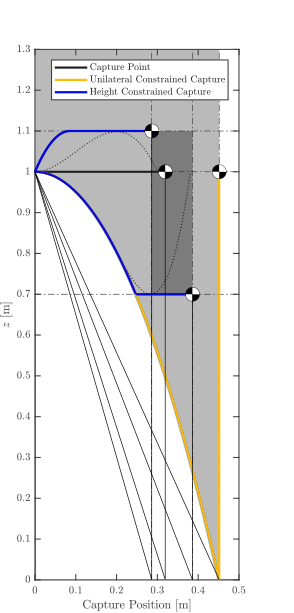
\includegraphics[width=3in]{STYLESTUFF/CPLimitsDark.png}
      \caption{Visualization of the analytic capture regions for $\dot{x}_0=1$ [m/s] and $\dot{z}_0=0$ [m/s]. The light gray area shows the unilateral contact constrained capture region (\ref{eq:xcpuni}). The dark gray area shows the height constrained capture region (Lemma \ref{lem:regionz})  for $0.7<z<1.1$ [m]. The dotted plots are made with the \textit{orbital energy controller} of \cite{koolen2016balance} and show that the final points are inside the height constrained region.}
      \label{fig:capregion}
\end{figure}

% Vertical Force
\section{Vertical Force Constraint}\label{sec:verticalforce}
If the assumption is made that the robot specific limitations on joint torques can be approximated with a minimum and maximum vertical force on the CoM. In doing so, constraints on the minimum and maximum vertical acceleration are added to the \ac{VHIP} dynamics. From Lemma 1, any vertical acceleration extremum at the earliest convenience will lead to staying closer to a height constrained bound. By inserting a constraint on vertical acceleration, an analytic solution for a capture position is not available anymore and needs to be solved numerically. The authors of \cite{gao2017increase} give analytic solutions using vertical acceleration, but consider a constant height in the model. For comparison with applied results later in this thesis, this constant height assumption is not considered
     
In \cite{pratt2006capture,stephens2007humanoid,koolen2012capturability}, a bang-bang control law is used to regulate the angular momentum in the body of model. Instead of using this strategy, a bang-bang control law is used to regulate the vertical acceleration:
\begin{equation}
	\ddot{z} = \ddot{z}_{c,1}H(t) - (\ddot{z}_{c,1} - \ddot{z}_{c,2})H(t-t_1) - \ddot{z}_{c,2}H(t-t_2),
\end{equation}
where $[\ddzcf,\ddzcs]$ are the first and second constant control inputs and have opposite signs. $H(\cdot)$ is the Heaviside step function and 
\begin{equation}
t_1=\sqrt{\frac{2(z_{const}-z_0)}{\ddzcf - \frac{\ddzcf^2}{\ddzcs}}},
\end{equation}
which is the solution of:
\begin{equation}
	z_0+\frac{1}{2}\ddzcf t_1^2 - \frac{1}{2}\frac{(\ddzcf t_1)^2}{\ddzcs}= z_{const},
\end{equation}
where $z_{const}=\zmin$ if $\ddzcf <0$ and $z_{const}=\zmax$ otherwise. The time $t_2=(1-\frac{\ddzcf}{\ddzcs})t_1$, as the second `bang` needs to drive the vertical velocity resulting from the first bang to zero. 
\begin{figure}
      \centering
      \includegraphics[width=3.2in]{STYLESTUFF/CPLimitsForce.png}
      \caption{Vertical acceleration constrained capture positions versus the height constrained bounds. The acceleration $\ddzc=|\ddzcf|=|\ddzcs|$ if $\ddzc \leq g$ and else the `bang' with the negative sign is set to $-g$.}
      \label{fig:zvsf}
\end{figure}

A binary search is used to find the capture positions with this control law. In Figure \ref{fig:zvsf}, simulation results are shown in perspective with the height constrained limits. Note that when the bang-bang control inputs are larger, both trajectory and capture position come closer to the height constrained bounds.

%% Cap comparison
\section{Capturability Comparison}
In this section, a comparison is made between the presented capture positions and the \ac{CP}, as well as a comparison with the \ac{LIP} plus flywheel capture regions. As in \cite{pratt2006capture, stephens2007humanoid, koolen2012capturability}, a \textit{dimensional analysis} is performed on comparing the capture regions. The following parameters are used for dimensionless position and velocity:
\begin{equation}
	x' = \frac{x}{z_0}, \qquad \dot{x}' = \frac{1}{\sqrt{gz_0}}\dot{x},
\end{equation}
The following dimensionless vertical acceleration, body inertia and \ac{CoM} torque are used:
\begin{equation}
 \ddot{z}'=\frac{\ddot{z}}{g}, \qquad I_y'=\frac{I_y}{mz_0^2}, \qquad \tau_y' = \frac{\tau_y}{mgz_0}.
\end{equation}
Instead of the \ac{CoM} torque, a dimensionless \ac{CMP} offset is used:
\begin{align}
	\xcmp' &=\frac{\xcmp}{z_0}=\xcop' + \delta \xcmp',\\
	\delta \xcmp' &=\tau_y',
\end{align}
where $\delta \xcmp'$ is the dimensionless \ac{CMP} offset. The dimensionless \ac{CoP} is assumed to be at a constant location.

\subsection{Evaluation of Capture Positions}\label{sec:capcomparenoinertia}
To make a comparison between the \ac{CP}, the height constrained capture positions and the vertical force constrained capture positions, the dimensionless vertical acceleration $\ddzc'$ of each `bang' for the vertical force constrained capture positions is set equal. For comparison, a rough estimate is made of realistic values of vertical forces that are achievable on both human and robot.

First, an approximation is made of what would be achievable for a human being. A human jumping vertically with maximum effort generates approximately $2mg$ ground reaction force \cite{linthorne2001analysis}. If the assumption is made that this value can also be used in recovery, we the value $\ddot{z}_c'=1$ can be taken for a human. Second, an approximation is made of what is possible on the robot. On hardware experiments on NASA's Valkyrie in Chapter \ref{chap:walking} is found that $\ddot{z}_c'=\frac{1}{4}$ is a well working value. Larger accelerations would result in the robot to shake and did not improve recovery. 

In Fig. \ref{fig:caplimits}, the height constrained bounds are shown, together with our approximations of what is realistic for vertical acceleration constraints on a human and on the robot. Note how the capture positions relate differently under a minimum height constraint than under a maximum height constraint. Also note how the capture position linking to the approximation of allowed vertical acceleration for a robot, seems to approach a minimum and maximum value quite soon after changing height. The point $[1,1]$ in the plot is the \ac{CP}.
\begin{figure}
      \centering
      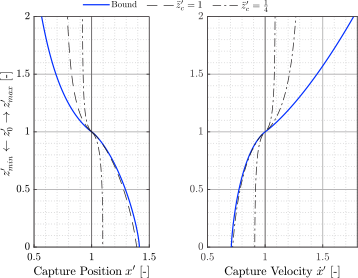
\includegraphics[width=5.2in]{STYLESTUFF/caplimits1.png}
      \caption{Plot of reachable dimensionless capture positions for $\dot{x}_0'=1$. }
      \label{fig:caplimits}
\end{figure}
\subsection{Comparison with Angular Momentum}
An estimation of the effects of angular momentum strategies can be performed as in \cite{koolen2012capturability}. Angular momentum strategies, like a `hip' strategy, have a pay back time; any angular velocity generated by the strategy has to be driven back to zero before a physical limit is reached. Therefore, the body torque can be estimated with a bang-bang control law.  Considering a \ac{LIP}, as proposed in the work mentioned, the following method is used to account for a angular momentum:
\begin{equation}
\delta\xcmp' = (1-2e^{-\delta \tbang'}+e^{-2\delta \tbang'})\delta \xcmpmax',
\end{equation}
where $\delta \xcmpmax'$ is the maximum dimensionless offset of the \ac{CMP} with the \ac{CoP} and $\delta \tbang'$ is the time of each ``bang'' of the control law. The average dimensionless \ac{CMP} offset to account for in computation of the \ac{CP} is $\delta \xcmp'$. The time $\delta \tbang'$ can be determined by:
\begin{equation}
\delta \tbang' = \sqrt{\frac{I_y'\theta_{max}}{\delta \xcmpmax'}},
\end{equation}
where $\theta_{max}$ the maximum allowed body lunge compared to the vertical. Note that $I_y'=0$ for a point-mass and $I_y'=1$ for a disc with all its mass on the edge, with its radius equal to the \ac{CoM} height above the ground. 

A rough estimate can be made of the dimensionless inertia of a human used in recovery. The assumption is made that the hip is the \ac{CoM} position and also the point of rotation for $J'$ and that the total body length is two times the \ac{CoM} height. Furthermore, only the body above the hip is assumed to be used in recovery, which is modeled as a beam with halve the total body mass rotating around an end: $I_{beam} = \frac{1}{3}(\frac{1}{2}m)L^2$. Note that the length $L$ is equal to the \ac{CoM} height $z$. Those assumptions result in the following dimensionless inertia:
\begin{equation}
	I_y' = \frac{\frac{1}{3}(\frac{1}{2}m)z^2}{mz^2} = \frac{1}{6}.
\end{equation}
Even though the inertia used in recovery is approximated with a calculation based on a beam, still a flywheel model is assumed. Rotation of a beam around its end would, in the case of a `hip' strategy, change the \ac{CoM} height of the system as well and would violate the \ac{LIP} model.

In \figref{fig:capcompare} the force constrained capture regions are compared with \ac{LIP} with flywheel capture regions. The maximum allowed vertical \ac{CoM} height change $\delta \zmax'$ is approximately the same value as is used on NASA's Valkyrie later in this report.
\begin{figure}
\centering
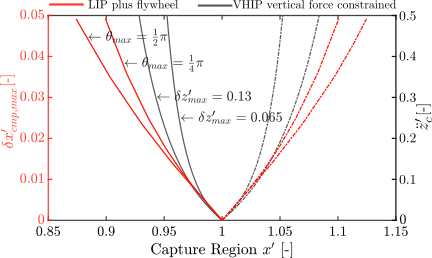
\includegraphics[width=0.9\textwidth]{STYLESTUFF/capcompare.png}
\caption{Comparison of capture region with angular momentum versus vertical force constrained capture. $\delta \zmax' =\delta \zmin'$ and $I_y' = \frac{1}{6}$.}
\label{fig:capcompare}
\end{figure}

%% Discussion
\section{Discussion}
In this chapter, different capture positions and capture regions for the \ac{VHIP} model are introduced. By comparing the capture positions, it can be observed how the addition of a constraint on the model can affect the capture region. Also, a high level comparison is made with angular momentum strategies.

Combination of height variation and angular momentum for balance recovery has two aspects worth mentioning. First, the \ac{GRF} in the phases with low or zero leg force will almost be orthogonal to the gravity vector if a hip torque is applied, which can cause slipping if ground friction is limited. Second, with lunging of the upper body, the \ac{CoM} will lower. In cases where height is increased for balance, this strategy is thus conflicting with use of angular momentum. Even maintaining a constant \ac{CoM} height may be difficult with lunging the upper body.

Friction cone..
%
% Another appendix chapter
\chapter{Orbital Energy MPC}
This \ac{MPC} method is based on the method of \cite{koolen2016balance}, which relies on \Eorbit~derived in \cite{pratt2007derivation}
\section{2D Polynomial}
Added a final velocity term $\dot{x_f}$ to the method of \cite{koolen2016balance}.
\begin{equation}
    \frac{1}{2}\dot{x}^2\bar{f}^2(x)+gx^2f(x) - 3g\int_{x_0}^xf(\xi)\xi d\xi = \frac{1}{2}\dot{x}_0^2\bar{f}^2(x_0)+gx_0^2f(x_0).
\end{equation}

\begin{equation}
    u = \frac{g + f''(x)\dot{x}^2}{\bar{f}(x)}
\end{equation}

\begin{equation}
    \underbrace{\begin{bmatrix}1 & 0 & 0 & 0 \\ 
     1 & x_0 & x_0^2 & x_0^3\\
     0 & 1 & 2x_0 & 3x_0^2\\
     \frac{3}{2}gx_0^2 & gx_0^3 & \frac{3}{4}gx_0^4 & \frac{3}{5}gx_0^5\\
     \end{bmatrix}}_A
     \underbrace{\begin{bmatrix}
     c_0\\
     c_1\\
     c_2\\
     c_3\\
     \end{bmatrix}}_{\boldsymbol{c}}=
     \underbrace{\begin{bmatrix}
     z_f\\
     z_0\\
     \frac{\dot{z}_0}{\dot{x}_0}\\
     k\\
     \end{bmatrix}}_{\boldsymbol{b}}
\end{equation}

where $k=\frac{1}{2}(\dot{x}_0z_0-\dot{x}_0x_0)^2 + gx_0^2z_0 - \frac{1}{2}z_f^2\dot{x}_f^2$.

Changing $\dot{x_f}$, changes the trajectory, which can be used in optimization.

% Height Constraint
\subsection{Height Constraint}
Maximum height. Algorithm \ref{alg:h}.
\begin{algorithm}
\caption{Find cubic polynomial constants under height constraint}
\label{alg:h}
\begin{algorithmic}[1]
\Procedure{FindPolZ}{$A^{-1},\boldsymbol{b}(\dot{x}_{f})$}
    \State $\dot{x}_{f}\gets 0$\Comment{Initial guess}
        \Repeat
            \State $\boldsymbol{c}\gets A^{-1}\boldsymbol{b}(\dot{x}_{f})$ \Comment{Find polynomial constants}
            \State $x_{zmax}\gets \frac{-2c_2 + \sqrt{4c_2^2-12c_3c_1}}{6c_3}$ \Comment{Traj. peak lies on highest x}
            \State $z_{max} \gets c_0 + c_1x_{zmax}^2 + c_2x_{zmax}^3+ c_3x_{zmax}^3$ \Comment{Corresponding height}
            \State $\dot{x}_{f} \gets \dot{x}_{f}+\alpha$   \Comment{Some smart increment}
        \Until{$z_{max}<z_{const}$}\\
    \Return $\boldsymbol{c}$
    \EndProcedure       
\end{algorithmic}
\end{algorithm}

\subsection{Leg Length Constraint}
Algorithm \ref{alg:ll}
\begin{equation}
(\sum_{n=0}^3 c_n x^n)^2 = \sum_{n=0}^3 c_n^2 x^{2n} + \sum_{\substack{n=1 \\ i+j=n \\ i < j}}^3 c_i c_j x^n 
\end{equation}
\begin{algorithm}
\caption{Find cubic polynomial constants under leg length constraint}
\label{alg:ll}
\begin{algorithmic}[1]
\Procedure{FindPolL}{$A^{-1},\boldsymbol{b}(\dot{x}_{f})$}
    \State $\dot{x}_{f}\gets 0$\Comment{Initial guess}
        \Repeat
            \State $\boldsymbol{c}\gets A^{-1}\boldsymbol{b}(\dot{x}_{f})$ \Comment{Find polynomial constants}
            \State $x_{lmax}^2 \gets \frac{-4c_2^2+\sqrt{16c_2^4-24c_3^2(2+2c_1^2)}}{12c_3^2}$ \Comment{$d(f(x)^2+x^2)/dx=0$}
            
            \State $x_{lmax}\gets-|\sqrt{x_{l^2max}}|$                \Comment{Complex solutions}
            \State $l_{max}^2 \gets x_{lmax}^2 + (c_0 + c_1x_{zmax}^2 + c_2x_{zmax}^3+ c_3x_{zmax}^3)^2$ 
            \State $\dot{x}_{f} \gets \dot{x}_{f}+\alpha$   \Comment{Some smart increment}
        \Until{$l_{max}^2<l_{const}^2$}\\
    \Return $\boldsymbol{c}$
    \EndProcedure       
\end{algorithmic}
\end{algorithm}

\subsection{Challenges 3D Orbital Energy}

\section{Results}
A planar walker that recovers from a push, where conventional \ac{CoP} control does not let it recover.

\section{Discussion}
2D..

%
% Another appendix chapter
\chapter{Toward Application: Walking}\label{chap:walking}
As the control strategy of Chapter \ref{chap:mpc} is in \ac{2D}, in this chapter a new strategy is proposed that is implementable on a real robot. First a experimental setup is shown with preliminary observations, to support assumptions made in the method developped. In the end, results are shown in simulation and on hardware.
% Experimental Setup
\section{Experimental Setup}
Evalutation of the strategy will be done based on push recovery on flat terrain. The situations considered when the push is applied are to be distinguished in two cathegories:
\begin{itemize}
	\item A static case, where the robot is standing
	\item A dynamic case, where the robot is walking
\end{itemize}
In both cathegories, limited foothold options are provided, such that step location adjustment would not be possible. Also, step timing is assumed to be given beforehand and is fixed, to make comparison with other control strategies more straight forward. The control strategies compared with are:
\begin{itemize}
	\item ``Ankle'' strategies: the desired \ac{CMP} is constrained to be inside the support polygon. 
	\item ``Ankle'' and ``Hip'' strategies : the desired \ac{CMP} can leave the support polygon uptil a maximum allowed distance.
\end{itemize}
The stepping parameters used for the walking test situation are given in Table \ref{tab:stepping}.
\begin{table}[ht]
\caption{Stepping Parameters} % title of Table
\centering % used for centering table
\begin{tabular}{c c c } % centered columns (4 columns)
\hline\hline %inserts double horizontal lines
Parameter & Value & Unit \\
%heading
\hline % inserts single horizontal line
Step Legth & 0.5 &  [m]\\
Step Width & 0.25 & [m]\\
\acs{SS} Time & 0.6 & [s]\\
\acs{DS} Time & 0.15 & [s]\\
%[1ex] % [1ex] adds vertical space
\hline %inserts single line
\end{tabular}
\label{tab:stepping} % is used to refer this table in the text
\end{table}
%Preliminary observations
\subsection{Preliminary Observations}
Before developping of a control method, the behavior of the system is studied, to get more insight in its behavior under handling errors. The following properties are observed after applying pushes on the robot from different directions in the experimental setups considered:
\begin{itemize}
	\item After a push in the swing phase, the direction of the \ac{ICP} error stays approximately the same until transition to \ac{DS}.
	\item If the \ac{ICP} error is directed in the sagittal plane, the desired \ac{CMP} often remains somewhat in the same location.
	\item if the \ac{ICP} error is directed  in the coronal plane, the desired \ac{CMP} slides from back to the forth of the foot.
	\item The configuration and velocity near transition to \ac{DS} affects the robots ability to put its swing leg down at the desired time. Also, the swing leg can collapse at touch down if the negative height velocity is too high.
	\item When the $\dotldz$ is high near the end of \ac{DS}, the robot can have problems with the transition to \ac{SS}.
\end{itemize}

\begin{figure}[h]
\centering
  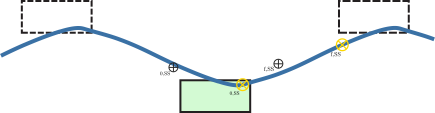
\includegraphics[width=.8\linewidth]{STYLESTUFF/ICPplan3StepComICPrSS.png}
   \caption{Initial (0,SS) and final (f,SS) configurations of \ac{CoM} position (black circle with cross) and \ac{ICP} reference (yellow circle with rotated cross) for \ac{SS} in the $xy$-plane with the parameters from Table \tabref{tab:stepping}. The green area is the current supporting foothold and the blue line is the \ac{ICP} reference trajectory.}
    \label{fig:3foot}
\end{figure}

\newpage
% Methods
\section{Methods}

%Strategy 
\subsection{Control Variables}\label{sec:strategy}

%
\paragraph{Alignment} of the line between $\rcopd$ and $\cxy$ with the vector $\icpe$ is used as a decision variable. If the vectors are perfectly aligned, $\ddzd$ will request $\dotldxyheight$ in the same direction as $\icpe$. This is, considering alignment, the perfect case to use height control. If the vectors are orthogonal, the requested $\dotldxyheight$ will be orthogonal to $\icpe$ and will not help driving back the error. Furthermore, the error in will grow in its orthogonal direction. Height control for any alignment in between the two cases mentioned will have a combined effect in resolving $\icpe$ in its direction, and generating additional error orthogonal to it.

\paragraph{Distance} in the horizontal plane between $\rcopd$ and $\cxy$ plays an important role in the effectiveness of height variation, \todo{secref}. As $\icpe$ and the virtual leg might not be perfectly aligned, the distance accounted for in the controller is the distance between the $\rcop$, and $\cxy$ projected on the line that is parallel to $\icpe$ and intersecting with $\rcopd$. In \figref{fig:phiViz} the alignment angle and the distance are visualized for different cases at entry of \ac{SS} for the test stepping parameters considered.

\begin{figure}[h]
  \begin{subfigure}{0.5\textwidth}
  \centering
  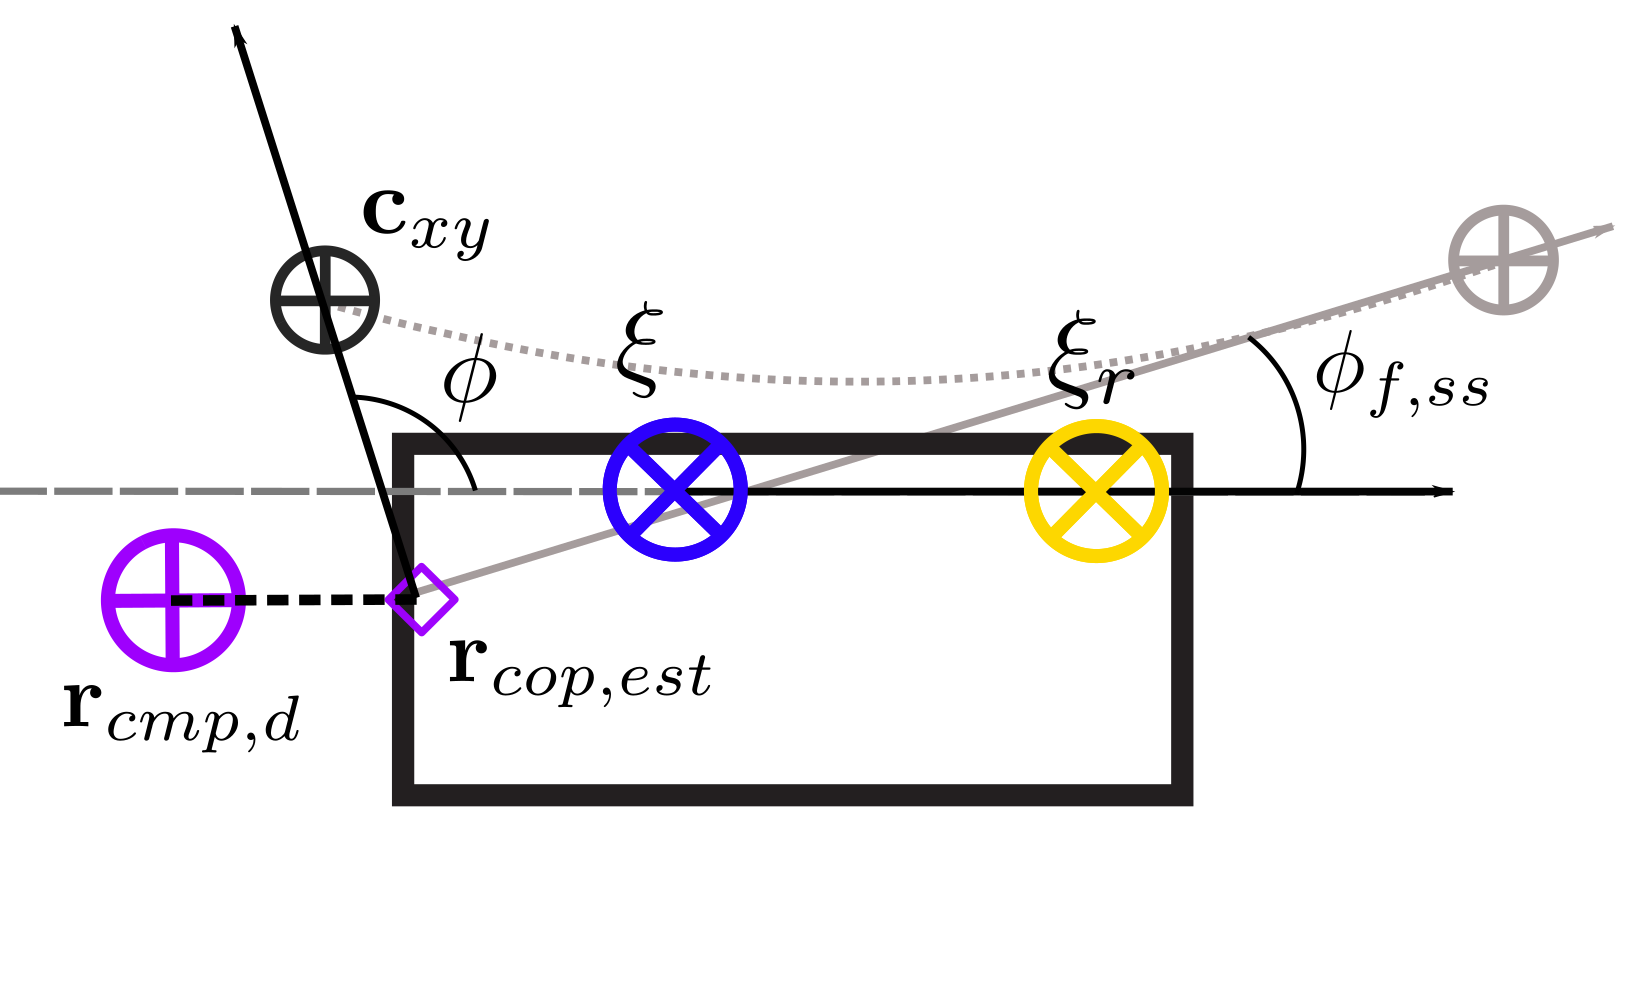
\includegraphics[width=.8\linewidth]{STYLESTUFF/ICPplanStartSSPhiViz.png}
   \caption{}
    \label{fig:phiViza}
  \end{subfigure}
  \begin{subfigure}{0.5\textwidth}
    \centering
  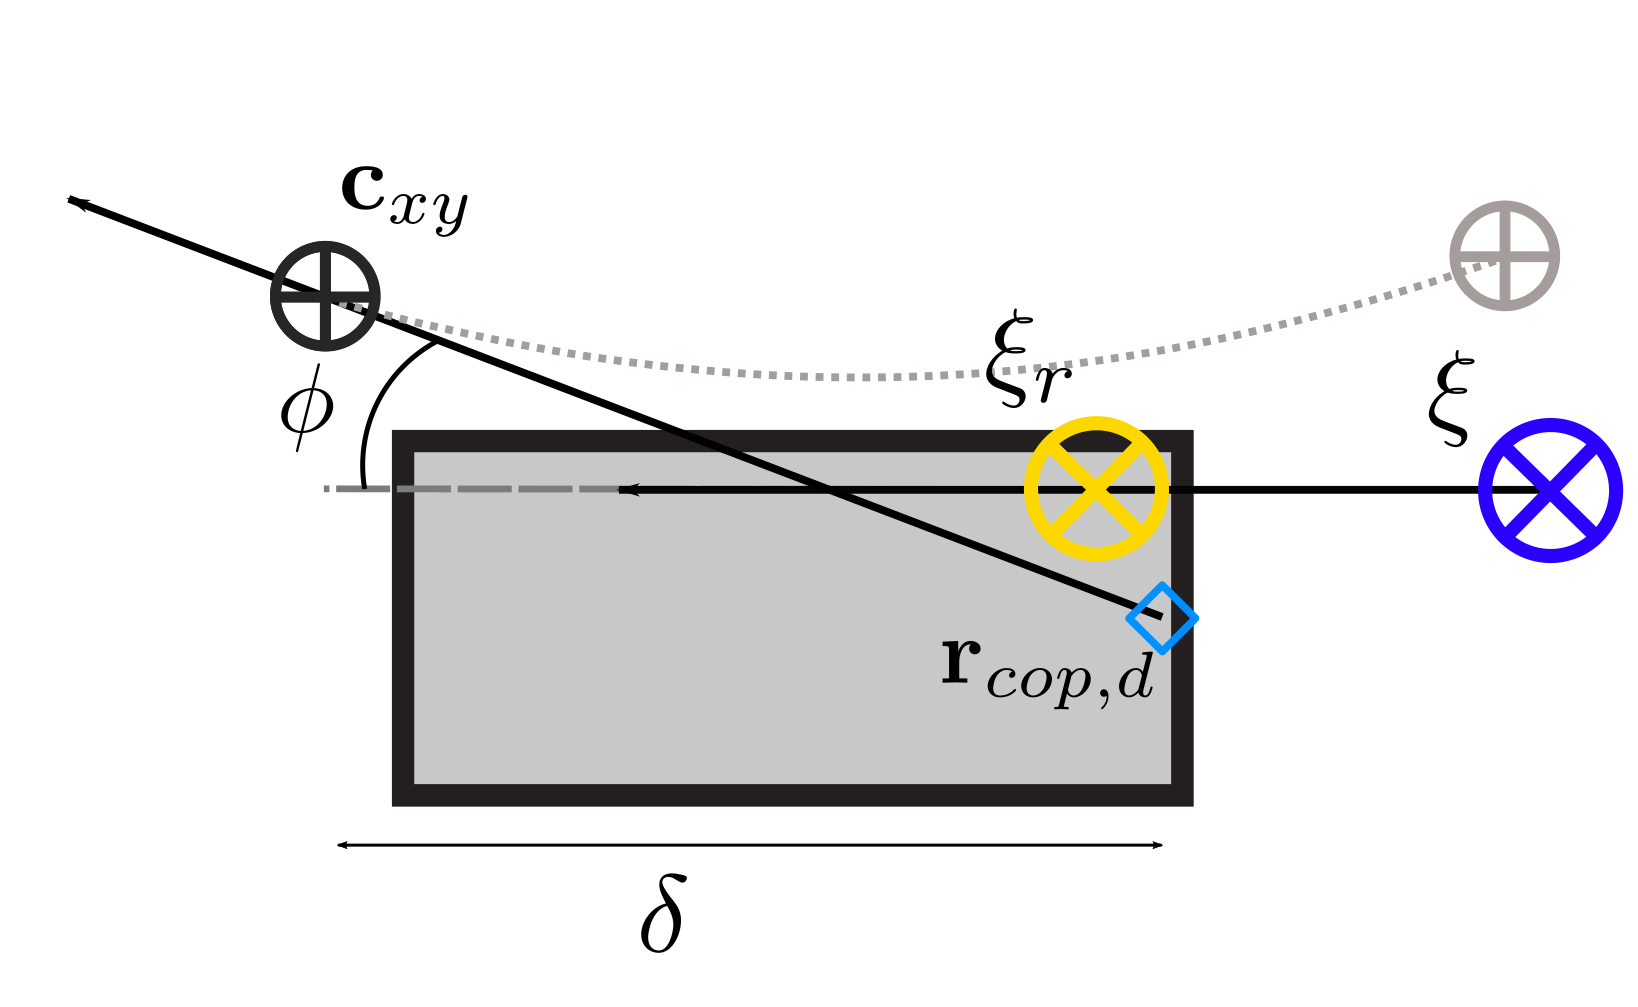
\includegraphics[width=.8\linewidth]{STYLESTUFF/ICPplanStartSSPhiVizNegError.png}
  \caption{}
   \label{fig:phiVizb}
  \end{subfigure}
  \begin{subfigure}{0.5\textwidth}
    \centering
  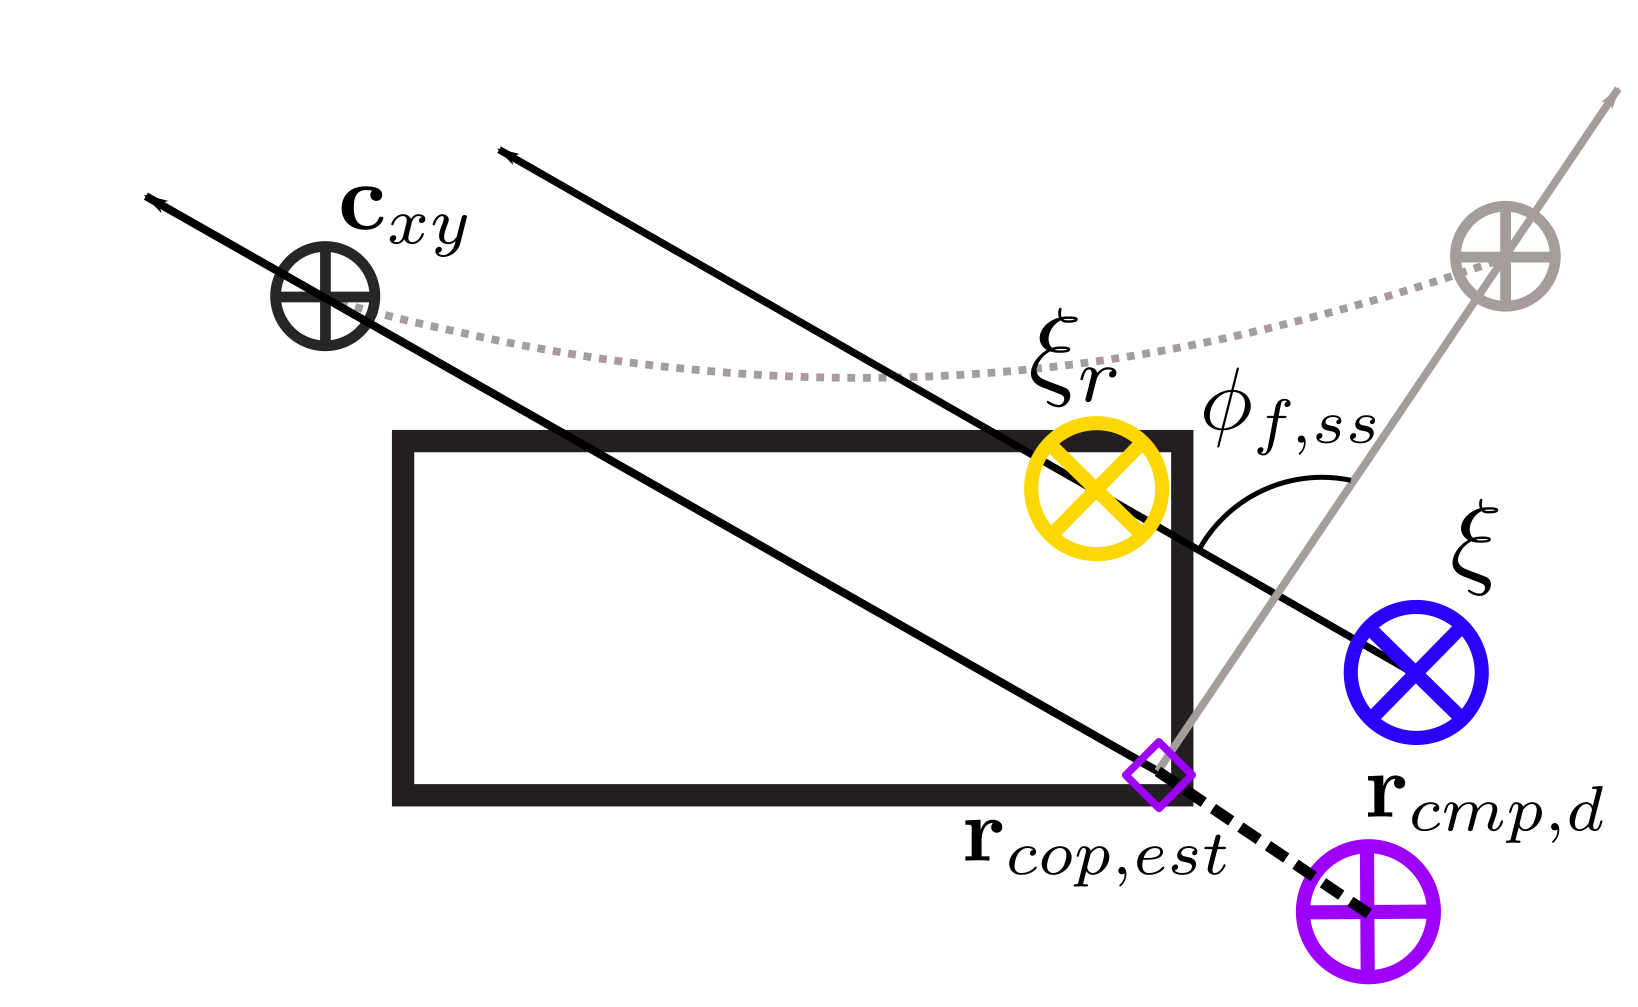
\includegraphics[width=.8\linewidth]{STYLESTUFF/ICPplanStartSSPhiViz0.png}
    \caption{}
     \label{fig:phiVizc}
  \end{subfigure}
  \begin{subfigure}{0.5\textwidth}
    \centering
  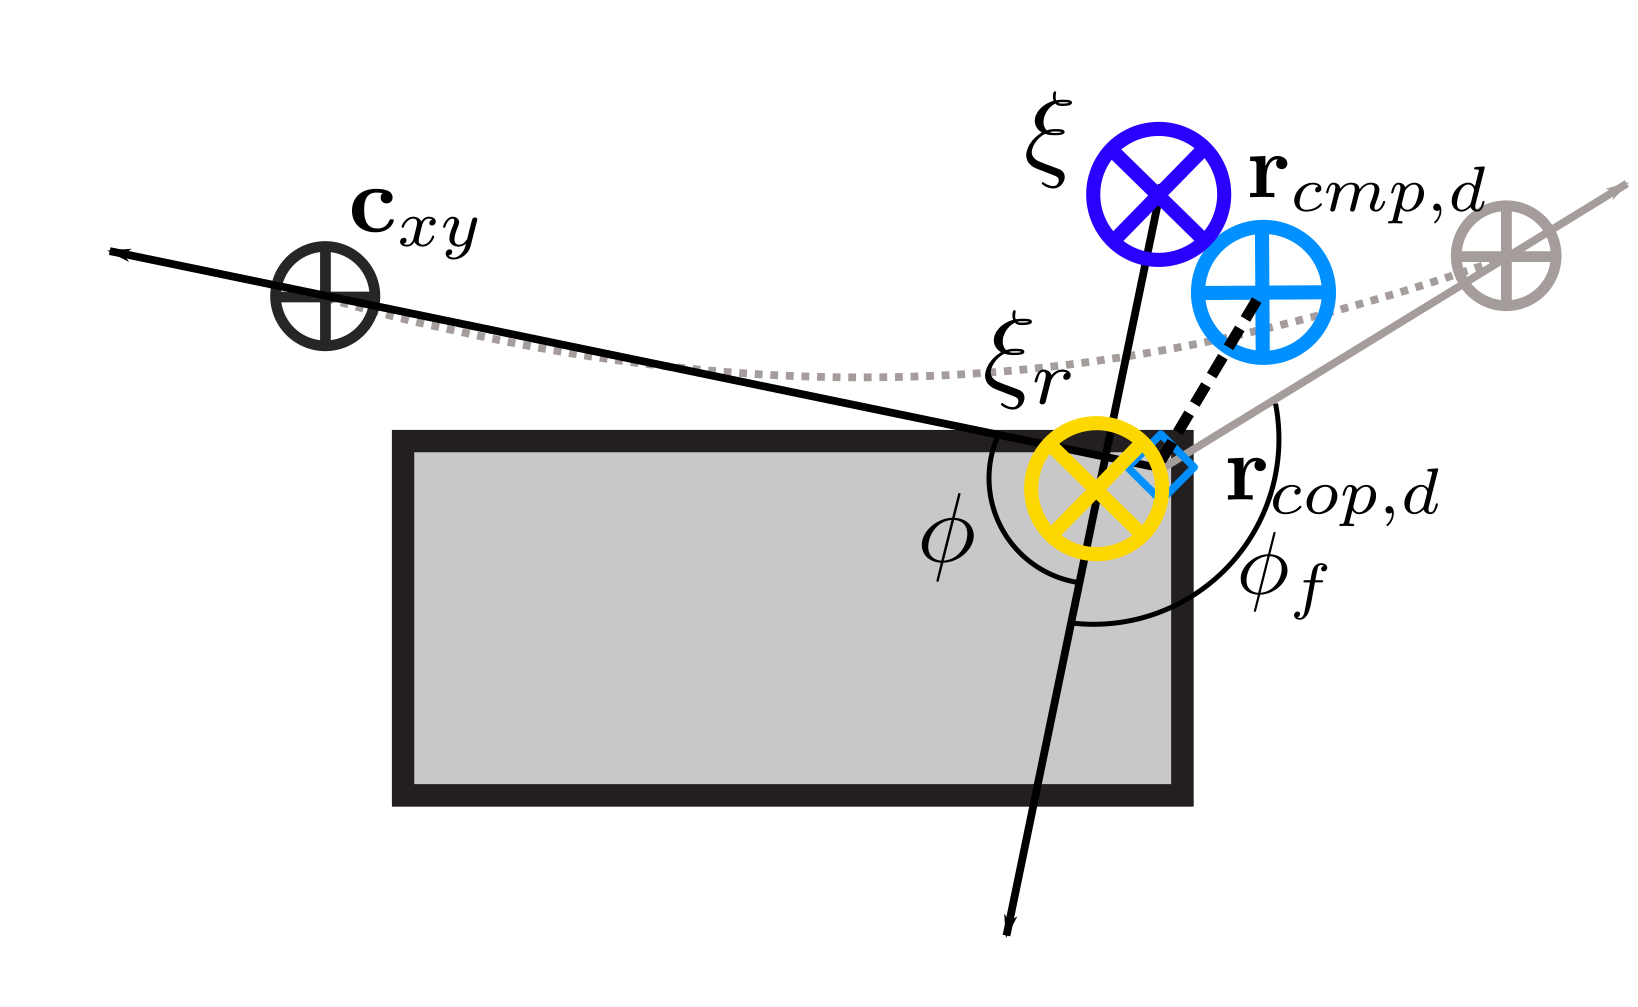
\includegraphics[width=.8\linewidth]{STYLESTUFF/ICPplanStartSSPhiViz90.png}
    \caption{}
     \label{fig:phiVizd}
  \end{subfigure}
    \begin{subfigure}{0.5\textwidth}
    \centering
  \includegraphics[width=.8\linewidth]{STYLESTUFF/ICPplanStartSSPhiVizLeftError.png}
    \caption{}
     \label{fig:phiVize}
  \end{subfigure}
  \begin{subfigure}{0.5\textwidth}
    \centering
  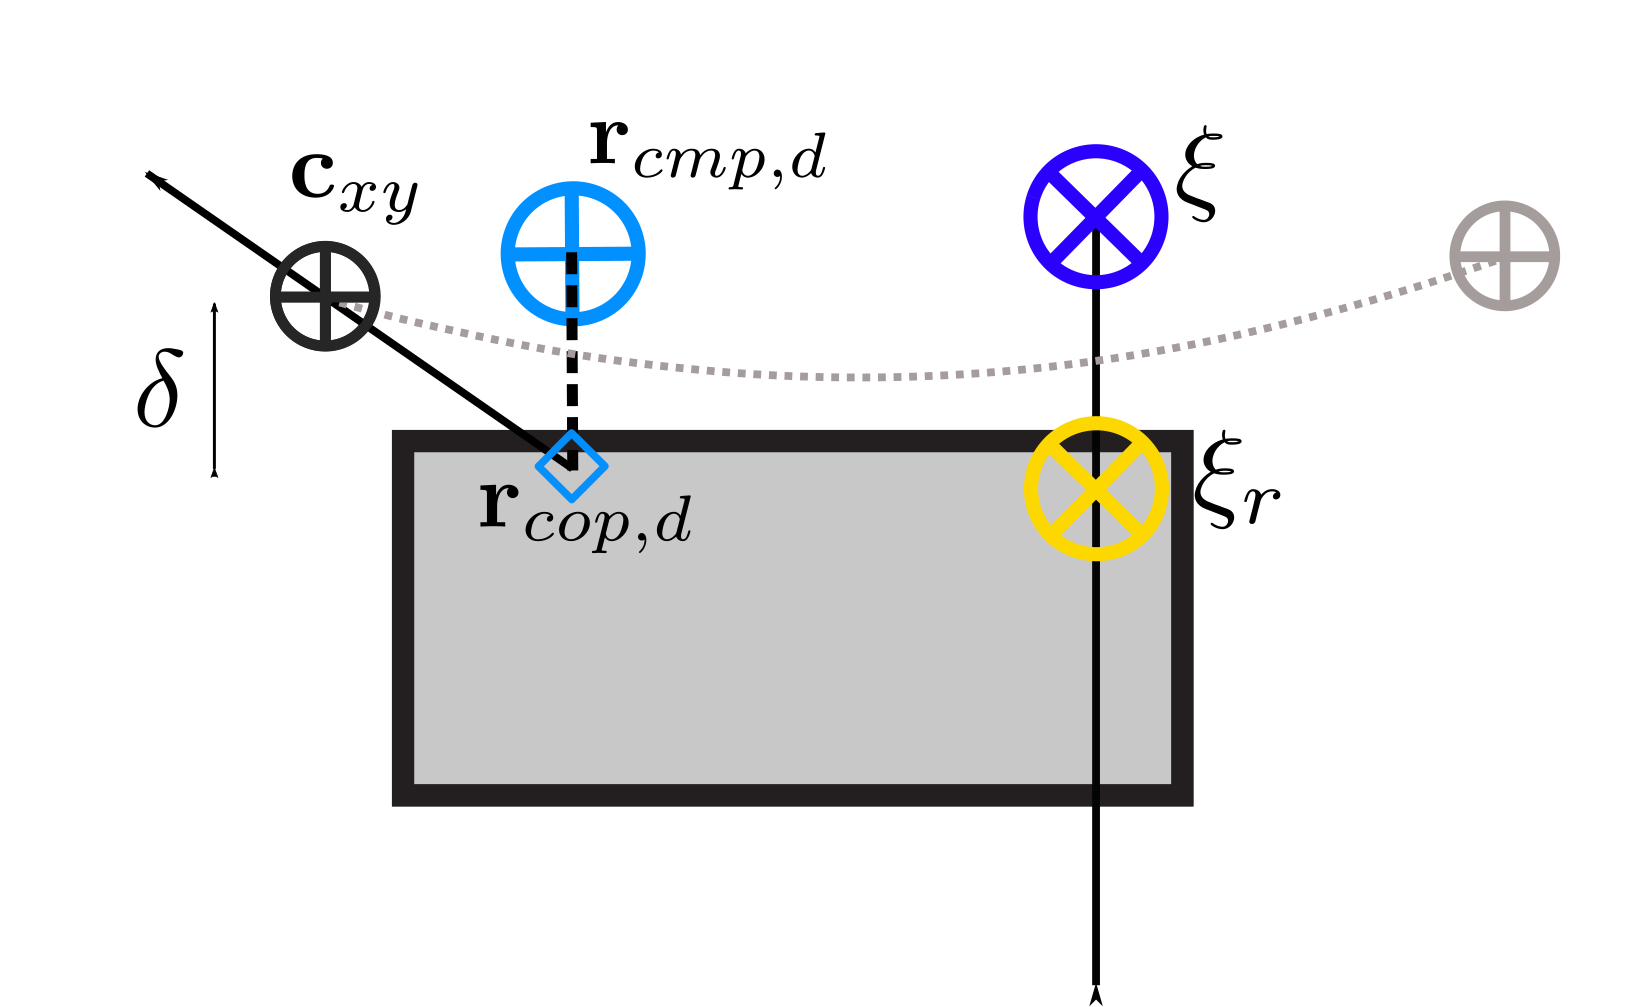
\includegraphics[width=.8\linewidth]{STYLESTUFF/ICPplanStartSSPhiVizRightError.png}
    \caption{}
     \label{fig:phiVizf}
  \end{subfigure}
  \caption{Vizualizations of the error alignment angle for the configuration at start of \ac{SS}, with \ac{ICP} errors: (a) negative in sagital plane, (b) positive in sagital plane, (c) where the error alignment angle is $0$ and (d) where the error alignment angle is orthogonal to the \ac{ICP} error.\todo{distance} }
  \label{fig:phiViz}
\end{figure}

\paragraph{The $\rcopd$ dynamics}

\paragraph{Constraints} that are considered are a minimum and maximum height and height velocity. The maximum length of the leg describes a part of a circle throught the swing phase. In the controller, this constraint is captured in two constraints: $\zmaxfirst$, in the first halve of the swing phase and $\zmaxscnd$, in the second part of the swing phase. In \figref{fig:heightconstraints} the two constraints are vizualized. 
\begin{figure}[h]
\centering
  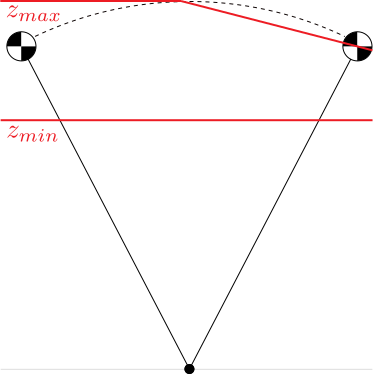
\includegraphics[width=.3\linewidth]{STYLESTUFF/heightconstraints.png}
   \caption{Height constraints through \ac{SS}}
    \label{fig:heightconstraints}
\end{figure} 
The predicted height the current state is about to reach is computed as:
\begin{equation}
	\zmaxpred = z + \sgn(\dot{z})\frac{\dot{z}^2}{-2\ddzminpred},
\end{equation}
where $\zmaxpred$ is the predicted maximum height from the current state and $\ddzminpred$ is the predicted maximum deceleration that will occur. This would be the gravity acceleration, but the minimal acceleration is limited. 
\paraskip
The minimum height constraint is not dependent on singularity of the swing leg and is kept at a constant value. Next to hitting the ground, a low height can cause problems at transfer to \ac{DS}, when the robot gets raised to default height again. The minimum height constraint $\zmin$ is displayed in \figref{fig:heightconstraints}. In a similar way as $\zmaxpred$, the minimum height constraint is computed as:
\begin{equation}
	\zminpred = z - \sgn(\dot{z})\frac{\dot{z}^2}{2\ddzmaxpred},
\end{equation}
where $\zminpred$ is the predicted minimum height from the current state and $\ddzmaxpred$ is the predicted maximum acceleration that will occur.
\paraskip
Contraints on the maximum height velocity $\dzmax$ and minimum height velocity $\dzmin$ are also taken into account. Reasons for this include collapsing of the swing leg at touch down and limited velocities at the robot. 



\paragraph{The time to the constraints} can also be computed, as a constant acceleration is considered. Time to maximum constraint, considered the minimum and maximum acceleration:
\begin{equation}
    z + \dot{z}\tzmax + \frac{1}{2}\ddzdmax\tzmax^2 + \frac{1}{2}\frac{(\dot{z} +\ddzdmax\tzmax)^2}{-\ddzminpred}= \zmax,
\end{equation}
where $\tzmax$ can be computed in the following way:
\begin{equation}
    \underbrace{\frac{1}{2}(\ddzdmax + \frac{\ddzdmax^2}{-\ddzminpred})}_a\tzmax^2 + \underbrace{(\dot{z} + \dot{z}\frac{\ddzdmax}{-\ddzminpred})}_b\tzmax + \underbrace{z - \zmax + \frac{1}{2}\frac{\dot{z}^2}{-\ddzminpred}}_c.
\end{equation}
Noting that $a$ is positive and that the time needs to be the positive solution, the predicted time to the maximum constraint reads as:
\begin{equation}
    \tzmax=\frac{-b + \sqrt{b^2 -4ac}}{2a}
\end{equation}
\paraskip
The predicted time to the minimum constraint is computed in a similar way:
\begin{equation}
    z + \dot{z}\tzmin + \frac{1}{2}\ddzdmin\tzmin^2 - \frac{1}{2}\frac{(\dot{z} +\ddzdmin\tzmin)^2}{\ddzmaxpred}= \zmin,
\end{equation}
where $\tzmin$ is computed as:
\begin{equation}
    \underbrace{\frac{1}{2}(\ddzdmin - \frac{\ddzdmin^2}{\ddzmaxpred})}_a\tzmin^2 + \underbrace{(\dot{z} - \dot{z}\frac{\ddzdmin}{\ddzmaxpred})}_b\tzmin + \underbrace{z - \zmax + \frac{1}{2}\frac{\dot{z}^2}{\ddzmaxpred}}_c.
\end{equation}
Noting that $a$ is strictly negative and that the time needs to be the positive solution, the predicted time to the minimum height constraint reads as:
\begin{equation}
    \tzmin=\frac{-b - \sqrt{b^2 -4ac}}{2a}
\end{equation}
\paraskip
The time to the maximum and mimimum velocity can be computed using a linear equation:
\begin{equation}
	\tdzmax = \frac{\dzmax - \dot{z}}{\ddzdmax}
\end{equation}
\begin{equation}
	\tdzmin = \frac{\dzmin - \dot{z}}{\ddzdmin}
\end{equation}

\subsection{Control Law}
\paragraph{Parameters}
\paragraph{Phases}


% Results
\clearpage
\section{Results}
Which cases? 
\begin{itemize}
	\item Normal limit v.s. height control on normal limit
	\item Normal limit v.s. height control limit -> capture limits? -> iterative push search.
	\item Angular momentum v.s. height control -> \todo{How?}
\end{itemize}
\subsubsection{Simulation}
\begin{itemize}
	\item 360 push: begin swing, half way swing, end swing.
	\item Front, back and diagonal pushes deeper evaluation.
\end{itemize}
On what?
\begin{itemize}
	\item ICP(t) v.s. ICPr(t) v.s. CoP(t) -> compare with assumptions
	\item Swing time and body pose.
\end{itemize}

\begin{figure}[h]
\centering
  \includegraphics[width=.3\linewidth]{STYLESTUFF/roundSSS.png}
   \caption{Height constraints through \ac{SS}}
    \label{fig:roundSSS}
\end{figure} 

\begin{figure}[h]
\centering
  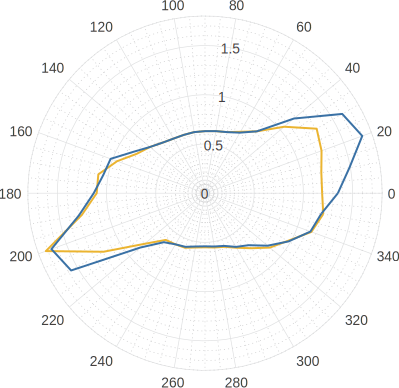
\includegraphics[width=.3\linewidth]{STYLESTUFF/roundHSS.png}
   \caption{Height constraints through \ac{SS}}
    \label{fig:roundHSS}
\end{figure} 
% Discussion
\section{Discussion}

%
% Another appendix chapter
\chapter{Conclusion}

\section{Recommendations}
\begin{itemize}
	\item Couple timeing adjustment with height control
\end{itemize}
%
%
%========================== Appendices =======================================
\appendix
%
%\include{app_another}

%========================== Back matter ======================================
\backmatter
%
% Bibliography
\bibliographystyle{ieeetr}
\printbib{MyBib}
%
%
% Glossary
\chapter{List of Acronyms} %
%
\printacronyms
\begin{acronym}[\hspace{0.8in}] % 0.8in is also used by the nomenclature
	\acro{3mE}[3\textlarger{m}E]{Mechanical, Maritime and Materials Engineering}%
	\acro{CoR}{Cognitive Robotics}%
	\acro{IHMC}{the Institute for Human and Machine Cognition}
	\acro{ICP}{instantaneous capture point}%
	\acro{CP}[LIPCP]{\ac{LIP} capture point}
	\acro{DCM}{divergent component of motion}%
	\acro{ZMP}{zero moment point}%
	\acro{CoP}{center of pressure}%
	\acro{CoM}{center of mass}%
	\acro{CMP}{centroidal momentum pivot}
	\acro{LIP}{linear inverted pendulum}%
	\acro{VHIP}{variable height inverted pendulum}
	\acro{2D}{two-dimensional space}%
	\acro{3D}{three-dimensional space}%
	\acro{MPC}{model predictive control}%
	\acro{SCS}{Simulation Construction Set}%
	\acro{SLIP}{spring-loaded inverted pendulum}%
	\acro{GRF}{ground reaction force}%
	\acro{SS}{single support}
	\acro{DS}{double support}
	\acro{QP}{quadratic program}
\end{acronym}%
%
%
% Nomenclature
%\printnomencl%

%
% Index
\cleardoublepage
\printindex

\end{document}
